
\documentclass{sigchi}

%% QUESTIONS FOR CHRIS AND ROB.

%% 1. Is Zooniverse the first citizen science project 
%%    to report scientific findings in research journals?
%% 2. XXX,XXX volunteers, NNN,NNN,NNN classifications
%% 3. ``Guide to social science papers'' - throw me a bone?
%% 

% Use this command to override the default ACM copyright statement (e.g. for preprints). 
% Consult the conference website for the camera-ready copyright statement.
\toappear{}

% Arabic page numbers for submission. 
% Remove this line to eliminate page numbers for the camera ready copy
%\pagenumbering{arabic}


% Load basic packages
\usepackage{balance}  % to better equalize the last page
\usepackage{graphics} % for EPS, load graphicx instead
\usepackage{times}    % comment if you want LaTeX's default font
\usepackage{url}      % llt: nicely formatted URLs
\usepackage{algorithm,algorithmic}
\usepackage{enumitem}


% llt: Define a global style for URLs, rather that the default one
\makeatletter
\def\url@leostyle{%
  \@ifundefined{selectfont}{\def\UrlFont{\sf}}{\def\UrlFont{\small\bf\ttfamily}}}
\makeatother
\urlstyle{leo}


% To make various LaTeX processors do the right thing with page size.
\def\pprw{8.5in}
\def\pprh{11in}
\special{papersize=\pprw,\pprh}
\setlength{\paperwidth}{\pprw}
\setlength{\paperheight}{\pprh}
\setlength{\pdfpagewidth}{\pprw}
\setlength{\pdfpageheight}{\pprh}

% Make sure hyperref comes last of your loaded packages, 
% to give it a fighting chance of not being over-written, 
% since its job is to redefine many LaTeX commands.
\usepackage[pdftex]{hyperref}
\hypersetup{
pdftitle={SIGCHI Conference Proceedings Format},
pdfauthor={LaTeX},
pdfkeywords={SIGCHI, proceedings, archival format},
bookmarksnumbered,
pdfstartview={FitH},
colorlinks,
citecolor=black,
filecolor=black,
linkcolor=black,
urlcolor=black,
breaklinks=true,
}


% create a shortcut to typeset table headings
\newcommand\tabhead[1]{\small\textbf{#1}}

% End of preamble. Here it comes the document.
\begin{document}

\title{One Does Not `Simply' Launch a Citizen Science Project: Reflections on Zooniverse, a Multi-Domain Science Platform}
% \title{A Brief History of Zooniverse: Designing for Multi-Domain Citizen Science}

\numberofauthors{1} \author{ (Authors removed for reviewing) }
% 
% Rob and Chris: please send me the complete list of authors on your team
% Zooniverse Team: Chris Lintott, Rob Simpson, Arfon (?) 
%   < insert main zooniverse team here > 
% 
% Southampton team: Max Van Kleek, Neal Reeves, Ramine Tinati, 
%   Elena Simperl, Anna Weston, Nigel Shadbolt, Wendy Hall (?)
% 


\maketitle

\begin{abstract}

(( TODO ))

\end{abstract}

\keywords{Citizen science, crowdsourcing, interface design}

%% TODO 
\category{H.5.m.}{Information Interfaces and Presentation (e.g. HCI)}{Miscellaneous}

%% TODO 
%% \terms{}

\section{Introduction}


While the tradition of amateur scientific discovery dates back at least two centuries, when citizen naturalists like Charles Darwin readily enlisted the help of friends and family in the pursuit of documenting flora and fauna around the world \cite{silvertown2009new}, the Internet has now democratised participation to a vastly greater scale and level of involvement.  Internet based citizen-science projects have brought scientific experiments to within reach of a few clicks of a mouse, enabling now millions of individuals to help in the midst of their everyday activities.

Examples of such projects, such as eBird \cite{wood2011ebird}, FoldIt \cite{khatib2011algorithm}, Old Weather \cite{}, and Stardust@Home \cite{westphal2005stardust} have already demonstrated that a crowdsourced approach to science can be valuable both to the participants, as educational tools and cognitively-stimulating puzzles \cite{gray2012lessons}, as well as to the original scientific research communities it was designed to serve. It offers a scalable, effective and accurate means to gather and analyse large data sets, and solve challenging problems, which, due to their size and complexity, remain difficult to master within existing scientific teams or with the support of state-of-the-art computational methods \cite{fortson2011galaxy,lintott2008galaxy,simpson2013dynamic}. % \cite{fortson-2011, lintott-08, lintott-11, simpson-12, davis-11}.

% "original?" - necessary?

Despite the successes achieved, citizen science systems remain notoriously challenging not only to design, but also to deploy and sustain (e.g. \cite{ebird, ubiome, druschke2012failures}). This is due not only to the novelty of the field, but also to the challenges intrinsically associated with the creation and effective support of online communities collaboratively pursuing research investigations. This scenario is arguably much more complex than other forms of crowdsourcing, such as microtask platforms such as Amazon's Mechanical Turk\footnote{Mechanical Turk - \url{www.amazon.com/mturk}}, which operate within a constrained set of mechanisms to accomplish tasks and interact, with a direct incentive scheme. By constrast, participants  interact with citizen science systems in many ways beyond performing tasks, such as by taking part in discussions, interacting with research teams, sharing interesting subjects, and so forth.  These many kinds of participation, in turn, reflect the many, varied, and often idiosyncratic motivations for taking part, the landscape of which is still being studied \cite{raddick2010galaxy}.

%such as...such as - Change? ALSO: "These many kinds of participation" -> "The many kinds of participation?"

% commented out: or challenges and open innovation, for instance InnoCentive\footnote{InnoCentive - \url{www.innocentive.com}}, which attract crowds many order of magnitudes smaller than most Zooniverse projects.

% hundreds of thousands of people engage with the system in many ways beyond performing the actual tasks; they take part in discussions, share items they found interesting, interact with professional research teams, and participate in the definition of new scientific workflows. This reflects the varied, and often idiosyncratic motivations that drive their volunteer efforts, the landscape of which is still only starting to be understood \cite{raddick2010galaxy}. 
% , often cited in the literature concerned with the development of sustainable online participatory systems in various domains (TODO references)

Even when such considerations have been made, citizen science systems can fail for many reasons. One important factor is the nature of the task to be crowdsourced. For some projects, the domain of the task may be intrinsically less interesting to members of the general public than others; in others, the task could turn out to be too difficult, requiring complex coordination or domain expertise. Other factors that could contribute to a project failing include aspects of the ways it is announced or launched, or the communication channels and resources allocated to provide community support over time.  Merely the ways that the community is structured to support such projects, including the ways moderators are chosen responsibilities they are given, could further influence long-term participation in the project as a whole. The combination of these factors means that designers must both cope with a high-dimensional, complex design space that is difficult to explore, resulting in outcomes that are unpredictable (e.g., \cite{ebird, ubiome, druschke2012failures}).

In this paper, we present an analysis of a citizen-science platform called \emph{Zooniverse} \footnote{Zooniverse - \url{www.zooniverse.org}}, which evolved from a one-time experiment in crowdsourced data analysis for astronomy, into a ``factory for citizen science'', a venerable authority for successful Web citizen-science applications across academic disciplines. Zooniverse-assisted scientific findings have been published in over 57 journal articles within both the natural sciences and the humanities, through the sustained effort of a dedicated and efficacious community of 864,482 volunteers as of September 2013.  This community has demonstrated a number of impressive achievements, from projects completing in the matter of days after launch (such as in Solar Storm Watch and the Andromeda Project), to citizens initiating and pursuing independent lines of inquiry based on curiosities they found in datasets, ultimately resulting in unanticipated scientific findings.  In terms of consistency, each of the 27 projects thus far launched have been attributed to producing at least one finding each, while some, such as the Galaxy Zoo family of projects, have produced dozens of findings alone.

While most of the specific discoveries made through Zooniverse have been documented elsewhere (e.g., \cite{lintott2008galaxy,lintott2009galaxy,story-of-the-peas,simpson2013dynamic}), the insights gained by the team through the iterative process of designing, deploying, and managing the over 27 citizen-science projects that have launched at the time of this writing have not previously been captured. To this end, we conducted a thematic analysis of insights and experiences gained by the Zooniverse team, which were elicited through a triangulation method that drew upon both qualitative and quantiative sources, including interviews with team members, discussion forums and blog posts, and classification databases.  Our objective was to identify the ways that the team's concrete experiences and project outcomes influenced the way they, in turn, designed and managed citizen science projects.  In so doing, we sought to understand the team's view on the citizen science's future, and gain an understanding of the HCI challenges that remained.

%the citizen science?

We begin with a brief introduction to Zooniverse, followed by a presentation of our results, framed in three themes: citizen-initiated discovery, factors influencing engagement, and launching a project.  Finally, we discuss the implications of these themes towards the design of new systems in terms of \emph{myths}, or anti-patterns, and discuss the Zooniverse perspective on crowd-science's future.

%We begin with aOur aim was to allow perspectives on the complicated design space in which citizen-science projects come into existence to be shared with both UX practitioners interested in designing such systems, as well as to contextualise these findings against the growing body of crowdsourcing and online community studies within HCI.

% Our case study will shed light on those aspects in the design and operation of citizen-science projects that have played a determinant role in the incredible success story behind Zooniverse. It will build upon the vast know-how of the Zooniverse team to define a set of guidelines and best practices in this emerging new field, which will inform the development of new systems that help resolve important research questions and sustain participation over time. As of today the Zooniverse team has been involved in $27$ citizen-science projects in natural sciences and the humanities, covering a wide variety of data sets and data analysis tasks. This project portfolio gives them a unique perspective on the many variations of needs pertaining to crowdsourced science, and extensive experience in designing and deploying such systems in production. The engineering of these systems followed an evolutionary, iterative approach, applying insights derived from each project to the next, with some projects being re-designed and re-launched several times. This process permitted the Zooniverse team to study design decisions at multiple levels, from the definition of the tasks the contributors are expected to undertake, to the tools by which members of the community interact with each other and with the science teams coordinating the projects, the user interfaces, and the strategies implemented when launching a new project or encouraging prolonged user engagement. 

%This project portfolio has given the Zooniverse team a unique perspective on the many variations of needs pertaining to crowdsourced science, and extensive experience in designing and deploying such systems in production.  The case study summarizes the findings of a retrospective reflective thematic analysis conducted with core members of the Zooniverse team, to identify the key design decisions that were made, and to document the informal knowledge gained across the various projects they have successfully launched and managed. Our aim was to allow perspectives on the complicated design space in which citizen-science projects come into existence to be shared with both UX practitioners interested in designing such systems, as well as to contextualise the underlying design dimensions against the growing body of crowdsourcing and online community studies being conducted in the HCI research community.


% We begin with a short history of the project in order to introduce readers to the broader context for the case study, followed by a dimensional design analysis of particular aspects of the design and deployment of Zooniverse projects.  Finally, we discuss the perspective of the Zooniverse team regarding the greatest difficulties they faced in building effective citizen science: $X$, $Y$ and $Z$, and ways that HCI research may be able to help.

% eMax's original > 
% Web-based ``citizen-science'' projects have enabled hundreds of thousands of untrained human volunteers to contribute to open scientific problems across a variety of domains \cite{citizen-science}.  The handful of successful systems have demonstrated that citizen science applications can be valuable both to participants, as educational tools and cognitively-stimulating puzzles \cite{citizen-science-in-curricula}, and as an invaluable method for tackling large problems and data sets \cite{fortson-2011, lintott-08, lintott-11, simpson-12, davis-11}.
%
% However, it can be extremely difficult to design successful citizen science systems that can achieve this mutually beneficial characteristic and that sustain participation over time.  The reasons are several: first, despite similarities with other kinds of human computation-driven systems, such as typical crowd-sourcing platforms like Amazon Mechanical Turk\footnote{Amazon Mechanical Turk \url{www.amazon.com/mechanicalturk}} or CrowdFlower\footnote{CrowdFlower \url{crowdflower.com}}, participants typically interact with with citizen science systems in many ways beyond performing tasks, such as by taking part in discussions, interacting with the science teams, sharing subjects they found interesting, and so forth.  These many ways that participants engage with citizen science systems reflects the many, varied, and often idiosyncratic motivations behind their reasons engaging with them, the landscape of which is still only starting to be understood \cite{raddick2010galaxy}.  % Designing to engage citizens along these many, personal reasons for participating requires an understanding of these motivations, the activities they foster, and ways to support these activities.
%
% Even when such considerations have been made, citizen science systems can fail for many reasons.  Often, these are due to factors essentially out of the control of the system designer; for example, for some projects, the domain subject matter or task may be intrinsically less interesting to members of the general population than others.  In some cases, the subjects being examined might be perceived as unpleasant, or even off-putting; tasks, for example, involving the identification of dead animals, or to locate parasites in  tissues of living patients may fall into this category.  Other factors that could contribute to a project failing include aspects of the ways it is announced or launched, or the communications channels and resources allocated to provide community support over time.  Merely the ways that the community is structured to support these projects, such as how moderators are chosen and the powers and responsibilities they are given, could further influence long-term participation in the project as a whole. The combination of these factors means that designers must both cope with a high-dimensional, complex design space that is difficult to explore, and outcomes that are quite unpredictable and uncertain (e.g., \cite{ebird, ubiome, druschke2012failures}).
%
% In this paper, we contribute a detailed case-study of a citizen-science platform called \emph{Zooniverse} \footnote{Zooniverse - \url{www.zooniverse.org}}, which expanded from a single domain experiment to a  ``factory for citizen science'', an authority for generating successful web applications for researchers across many domains.  Zooniverse projects have thus far (as of September 2013) resulted in the publication of findings in over (TODO -- $57$) journal articles, contributing findings to astrophysics, zoology, archaeology, cell and marine biology and climatology.  It has also developed and sustained a dedicated and efficacious user community, that pursue (and often complete) new projects and data sets soon after they are introduced.  Perhaps of most significance, several Zooniverse projects have benefited from \emph{citizen initiated} serendipitous discoveries which have resulted in bi-directional collaborative processes between the volunteers and the science teams, for evidence collection, hypothesis generation, and validation.%  
% This experience given the Zooniverse team a unique perspective on the many variations of needs pertaining to citizen science problems, and extensive experience in designing and deploying such systems in production. These projects followed an evolutionary, iterative design process, applying insights derived each project to the next, with some projects re-designed and re-launched several times.  This process permitted the team to explore design decisions at multiple levels, from the interface/task design level, to the design of discussion forums, to launching and involvement strategies for sustaining prolonged engagement. 
%
% In this paper, we summarise the results of a retrospective reflective thematic analysis conducted with core members of the Zooniverse team, to identify the key design decisions that were made, and to document the informal knowledge gained from their process.  This was done primarily to allow perspectives on this complicated design space to be shared with both UX practitioners interested in designing for citizen-science, as well as to contextualise these design dimensions against the growing crowd-sourcing and online community studies being in the HCI research community.  
% We begin with a short history of the project in order to introduce readers with the context for the following discussion, followed by a dimensional design analysis of particular aspects of Zooniverse's deployment.  Finally, we discuss Zooniverse's team's perspective of the greatest difficulties for building more effective citizen science: $X$, $Y$ and $Z$, and ways that HCI research may be able to help.

\section{Background}
\begin{table*}
\begin{center}
\small
\begin{tabular}{lcllclll}
\hline
Project & Status & URL & Launch & Domain & Logged-In & Subjects & Task \\
Name &  &  & Date &  & Users &  &   \\
\hline
\hline
Galaxy Zoo & Retired & zoo1.galaxyzoo.org & 11 Jul 2007 & Space & 165,000 & 890,000 & Classifying \\
\hline
Galaxy Zoo 2 & Retired & zoo2.galaxyzoo.org & 16 Feb 2009 & Space & 223,965 & 304.122 & Classifying \\
Galaxy Zoo Mergers & Retired & mergers.galaxyzoo.org & 23 Nov 2009 & Space & 20,588 & 58,956 & Classifying \\
\hline
Solar Stormwatch & Active & solarstormwatch.com & 22 Feb 2010 & Space & 65,971 & YY,YYY & Classifying/Marking \\
Galaxy Zoo Supernova & Retired & supernova.galaxyzoo.org & 26 Mar 2010 & Space & 37,150 & 76,376 & Classifying \\
Galaxy Zoo: Hubble & Retired & zoo3.galaxyzoo.org & 17 Apr 2010 & Space & XX,XXX & ~200,000 & Classifying \\
Moon Zoo & Active & moonzoo.org & 11 May 2010 & Space & 121,251 & 435,314 & Marking \\
Old Weather & Active & oldweather.org & 12 Oct 2010 & Climate & 32,076 & YY,YYY & Transcribing \\
The Milkyway Project & Active & milkywayproject.org & 07 Dec 2010 & Space & 57,675 & 35,695 & Marking \\
Planet Hunters & Active & planethunters.org & 16 Dec 2010 & Space & 167,354 & 3,063,759 & Marking \\
\hline
Ancient Lives & Active & ancientlives.org & 25 Jul 2011 & Humanities & 24,983 & 153,885 & Transcribing \\
Ice Hunters & Retired & icehunters.org & 09 Aug 2011 & Space & 15,276 & YY,YYY & Classifying/Marking \\
NEEMO & Active & neemo.zooniverse.org & 15 Oct 2011 & Space & X,XXX & YY,YYY & Classifying \\
Whale FM & Active & whale.fm & 29 Nov 2011 & Nature & 2,150 & 15,531 & Classifying \\
\hline
SETI Live & Active & setilive.org & 29 Feb 2012 & Space & 63,609 & 27,004 & Classifying \\
Galaxy Zoo 4 & Active & galaxyzoo.org & 11 Sep 2012 & Space & 48,550 & 390,907 & Classifying \\
Seafloor Explorer & Active & seafloorexplorer.org & 13 Sep 2012 & Nature & 14,099 & 123,077 & Marking \\
Cyclone Center & Active & cyclonecenter.org & 27 Sep 2012 & Climate & 4,767 & 196,638 & Classifying \\
Bat Detective & Active & batdetective.org & 02 Oct 2012 & Nature & 1,580 & 582,203 & Classifying \\
Cell Slider & Active & cellslider.net & 23 Oct 2012 & Biology & 13,261 & 275,702 & Classifying \\
Andromeda Project & Active & andromedaproject.org & 05 Dec 2012 & Space & 5,072 & 12,425 & Marking \\
Snapshot Serengeti & Active & snapshotserengeti.org & 11 Dec 2012 & Nature & 22,173 & 1,240,727 & Classifying \\
\hline
Planet Four & Active & planetfour.org & 08 Jan 2013 & Space & 34,718 & 98,920 & Marking \\
Notes from Nature & Active & notesfromnature.org & 22 Apr 2013 & Nature & 3,490 & 123,402 & Marking/Transcribing \\
Space Warps & Active & spacewarps.org & 08 May 2013 & Space & 9,544 & 345,240 & Marking \\
Worm Watch Lab & Active & wormwatchlab.org & 30 Jun 2013 & Biology & 3,251 & 74,016 & Classifying \\
\hline
\end{tabular}
\normalsize
\label{table:project-summary}
\caption{Summary of Zooniverse projects past and present, including each projects status as of September 2013.  The 1.68 million assets in the various Galaxy Zoo projects are not unique, since galaxies in GZ1 were used in subsequent projects.}
\end{center}
\end{table*}

% According to neemo.zooniverse.org, NEEMO had 47,943 user validations, though this may differ from "logged-in users." Particularly because two figures are given - 485 volunteers joined the mission.
Citizen-science systems be broadly categorised into those concerned with data collection (e.g., \cite{zook2010volunteered,wood2011ebird}), data analysis (e.g. \cite{westphal2005stardust,heinzelman2010crowdsourcing}), and problem-solving (e.g., \cite{khatib2011algorithm,cordero2012rna}).  Zooniverse projects fall into the \emph{data analysis} category.  Data, comprising, digital artifacts such as images, video and audio recordings, typically captured by cameras, telescopes and other equipment, are analysed by volunteers, who identify, classify, mark and label the phenomena that appear in them according to instructions given by the science team. As documented previously by Fortson et al \cite{fortson2011galaxy}, the first Zooniverse project, \emph{Galaxy Zoo}\footnote{Galaxy Zoo - \url{www.galaxyzoo.com}}, launched July 2007, engaged volunteers in the morphological classification of images of galaxies \cite{galaxyzoo-launch}. The early success of Galaxy Zoo (reaching more then 100,000 users by 2008) led the project team to branch out to new domains and task types. 

%information generated by the crowd soon resulted in scientific papers on spin statistics of spiral galaxies\cite{land2008galaxy} and the morphological characteristics of galaxies\cite{lintott2008galaxy}. The success of Galaxy Zoo generated significant interest, and it became clear that there would be more projects to follow.  The first such project was \emph{Solar Stormwatch}\footnote{Solar Stormwatch - \url{www.solarstormwatch.com}}, effectively built for the Royal Observatory of Greenwich by Zooniverse.  The first non-astronomy project, \emph{Old Weather}\footnote{Old Weather - \url{www.oldweather.org}}, launched in October $2010$ and asked volunteers to transcribe historical, hand-written weather measurements from official logs of merchant trading ships from the period of $1780$ to $1830$.  As of September $2013$, the Zooniverse family of projects has benefited from the participation of $864,482$ volunteers who have collectively submitted over $NNN,NNN,NNN$ contributions across different projects to the system.

Table \ref{table:project-summary} lists all Zooniverse projects by their launch date, and indicates their status, web address, subjects being processed, and task type\footnote{all statistics are as of September 2013; the active projects may be extended to new data sets so the number of subjects is likely to increase through time}. \emph{Retired} projects have achieved their classification goals and have been closed for new contributions. \emph{Active} projects are those still open for new contributions.  Projects generally have one or task type; \emph{classifying} tasks ask users to identify the presence, types, and potentially number of √items visible in each subject.  \emph{Marking} tasks involve the additional step of indicating the location of the particular object in the image.  Finally, \emph{transcribing} tasks require reading ancien texts and typing them in, such as the ship logs in \emph{Old Weather}. Figure 1, likewise, illustrates the growth of the project from June 2007 until September 2013.  

At the time of writing, results from Zooniverse projects have been documented in over 279 scholarly articles, with 57  dedicated to Zooniverse findings; 39 publications have resulted from Galaxy Zoo alone.  Pertaining to studies of Zooniverse as a whole, Raddick et al conducted an interview study to understand the motivations of Zooniverse volunteers \cite{raddick2010galaxy}. For additional information we refer to reader to the Zooniverse blog, which has a complete list of publications across all the Zooniverse projects \cite{zooniverseblog}.

\subsection{Overview and Teminology of the \emph{Zooniverse}}
In this paper, we adopt the Zooniverse team's terminology for describing their citizen-science platform, which we briefly introduce here. The Zooniverse platform contains a set of core technology components, which can be instantiated in various forms and combinations to run specific \emph{projects} with their own scientific tasks and data sets. Such projects are proposed to the Zooniverse team by researchers, who become the project's \emph{science team}.  The science team are ultimately responsible for the project once launched; this spans the provisioning of the data to be analyzed by the crowd, but also community engagement activities. Each project represents a single, specific line of inquiry and data set, and is launched as a separate Web site, with a dedicated discussion forum,  and associated social media channels, including a blog, a Twitter account, and a Facebook page.  Volunteer participants are referred to as \emph{users}. Once signed-up they can contribute to any of the Zooniverse projects; each of these projects displays links to other projects in the Zooniverse family at the top of their Web site.

Users who participate in Zooniverse projects extensively may be rewarded with moderator status, or mentioned in blog articles written by the science team, but are not otherwise incentivised.  Moderators are given privileges such as the ability to freely move, delete, and edit posts in forums, and visible indicators next to their display avatars; they are also the only users given access to contact the \emph{science teams} in charge of the project. The term \emph{subject} refers to the individual assets that users are tasked with analyzing.  Subjects may come in different forms, such as images, audio files and videos. \emph{Tasks} are the particular activities which users carry out when presented with a subject, such as identifying the presence and shape of a galaxy in a set of subjects. The generic term for such a galaxy would be \emph{object} - in other words, users analyze a subject (e.g., an image) to find, classify, mark, or label objects contained by the subject. Subjects are typically organised into \emph{groups}, which represent a particular data set collection, such as those from a particular time period or source such as the Hubble telescope.  Finally, a \emph{Classification} is a single classifying, marking or transcribing action performed by a single user, upon a subject, within the context of some task, of a project.

% \subsection{Previous Zooniverse Studies}
% (( TODO : Write up a summary of the social science and systems Zooniverse papers ))

\section{Method}

\begin{figure}[tbp]
\begin{center}
\begin{enumerate}[itemsep=1mm]
\item \emph{When you design and launch a new project now, what do you do differently than you would done at the start?}
\item \emph{Were there any surprises, or unexpected outcomes?}
\item \emph{What made projects most and least successful?}
% \item \emph{What were your best ideas and worst mistakes?}
\end{enumerate}
\vspace{10pt}
\caption{\emph{Probes for triangulation} - The interview process started with (and iteratively returned to) these four main questions as probes, to yield the main themes for analysis.}
\label{tbl:questions}
\end{center}
\vspace{-18pt}
\end{figure}

% Our objective was to identify the ways that the team's concrete experiences and project outcomes influenced they way they, in turn, designed and managed citizen science projects.  In so doing, we sought to understand the team's view on the 

To identify the insights that most influenced the decisions the team made when designing, launching and conducting new projects, we adopted a mixed-method triangulation approach \cite{olsen2004triangulation} drawing from qualitative and quantitative sources. Interviews were conducted with the core members of the Zooniverse team, comprising the lead project founder, team architect, and two members of the Galaxy Zoo design team.  These individuals were selected because they were instrumental to both the beginnings of Zooniverse, and because they were responsible for key design and strategy decisions throughout.  Interviews were loosely based around a set of questions (see Table \ref{tbl:questions}) that were designed to elicit reflections on the process and identify what was learnt along the way.   We conducted four interview sessions, two on one day, and two after the results of the first day were thematically arranged using an iterative grounded thematic analysis \cite{mazzolini2003sage}.  While the goal of the first was to generate potential themes, the second focused on validation and in-depth understanding of the themes described.  Prior to the interviews, and during thematic analysis, several other sources were consulted, including discussion boards for four Zooniverse projects, \emph{talk pages} for thirteen projects, as well as twenty six Zooniverse-related blogs. 
% These two individuals oversaw the design, development, launch, and management of the projects, and coordinated with specialised science teams on the post-processing of data and derivation of scientific results, as well as leading in several published findings.  

% TODO:
% FILL IN XXX ABOVE

% The study also drew upon a mix of quantitative data sources including Galaxy Zoo Forums, and a snapshot of the entire Zooniverse Talk system and classification databases. Included within these snapshots were the records for each individual user (anonymised), the classification for (n) different Zooniverse projects, and the individual comments made of the discussion forums of the respective Zooniverse projects. The purpose of using this mixed methods approach was to compliment and add further insight into the rich qualitative data sources \cite{EdwardsCrossley2009} in order to further unpack and understand the characteristics of producing successful Citizen Science projects.

% Quantitative sources we drew upon included the launch histories, google analytics logs, and classification databases for all the projects.  The project launch curves were used to gain an understanding of the various trajectories of the projects, and to ask drive a discussion about the factors that influenced each.  Themes were derived from project performance curves and timelines, and these were used for a second round of interviews with the team leaders around these themes.

% triangulation approach?
% In order to identify the insights most valuable to the team from their multi-year iterative design process, we applied a mixed-methods approach drawing upon both quantitative and qualitative sources. The qualitative data collected consisted of four semi-structured interviews, conducted with the Zooniverse lead project manager and team lead architect. Interviews were chosen as the main source of qualitative data for this study for a number of reasons, they provide a rich and first-hand source of information which can help to draw out insights unlike other sources of qualitative or quantitative data \cite{Yin2003}, to this point, the tacit knowledge that this paper wishes to describe is embedded within the experiences gained within the Zooniverse team members. Interviews provide the unique position where more than one set of experiences and opinions can be discovered, and it is through the triangulation and agreement between data sources that help distill rich insightful \cite{Denzin1978} \cite{Morse1994}. 

% The interviews were conducted over a serious of four 2-hour digitally-recorded sessions. Each participant was asked identical open-ended questions, visible in Table \ref{tbl:questions} related to their experience in designing, launching, and maintaining the citizen science projects which they have been involved in. The interviews were performed in two, 2-hour sessions as part of a reflective process to ensure that the interviewee had had adequate time to describe and reflect on their experiences discussed. Prior to the initial interview session, the participants were asked to prepare any material they wished (in various mediums, i.e. text, video, presentations) which would help them capture the previous 5 years of experience which they have gained during the design, development and deployment cycle of the citizen science projects they were involved with. At the end of the first session, the manually transcribed dialogue were given to the participants in order for them to reflect on the experiences which they shared. The second session was then used to discuss these experiences in more detail which were captured in additional notes taken by the researcher. After the second stage of interviews, the transcripts were amended where required, and then anonymised in order to ensure integrity within the coding and elicitation stages of the study. The reflective iterative process used within this study was found to help extract experience and knowledge of the participants which would have remained hidden without the chance for interviewees to comment and discuss their dialog further. It was also found that participants use of material within the were beneficial for helping them recall experiences, especially with regards to the earlier Zooniverse projects.

% Within the what?
% An iterative manual coding approach was conducted by three researchers to provide the first level of analysis for the interviews. In order to initiate the coding process a topic guide was used which contained themes related to the questions that interviewees were asked. Each interview underwent a first iteration of coding based upon the codes within the topic guide, and during this process additional themes were identified. This process was performed by the 3 researchers who subsequently cross-compared the additional themes they each found. Based upon an agreement of these new themes and a review of the notes that were taken by the researcher that conducted the initial interview, a new coding schema was developed and the interviews were re-coded in order to extract codes that were missed. This process was repeated for each interview in order to ensure validity and consistency \cite{Strauss1987} \cite{Lafaille1995}. Each researcher also took notes when coding the interviews to describe any comments or discussions that appeared relevant but external to the themes identified. Separate coding of the interviewees were brought together using NVIVO which was then used to extract the relevant information required.

\section{Results: Key Themes}
%% TODO: three themes? how many 
In this section, we present the results of our analysis around the themes of \emph{citizen-led discoveries}, \emph{dimensions of engagement} and \emph{project launches}.

\subsection{Citizen-led Investigations and Serendipitous Discoveries}

\begin{figure}[htbp]
\centering
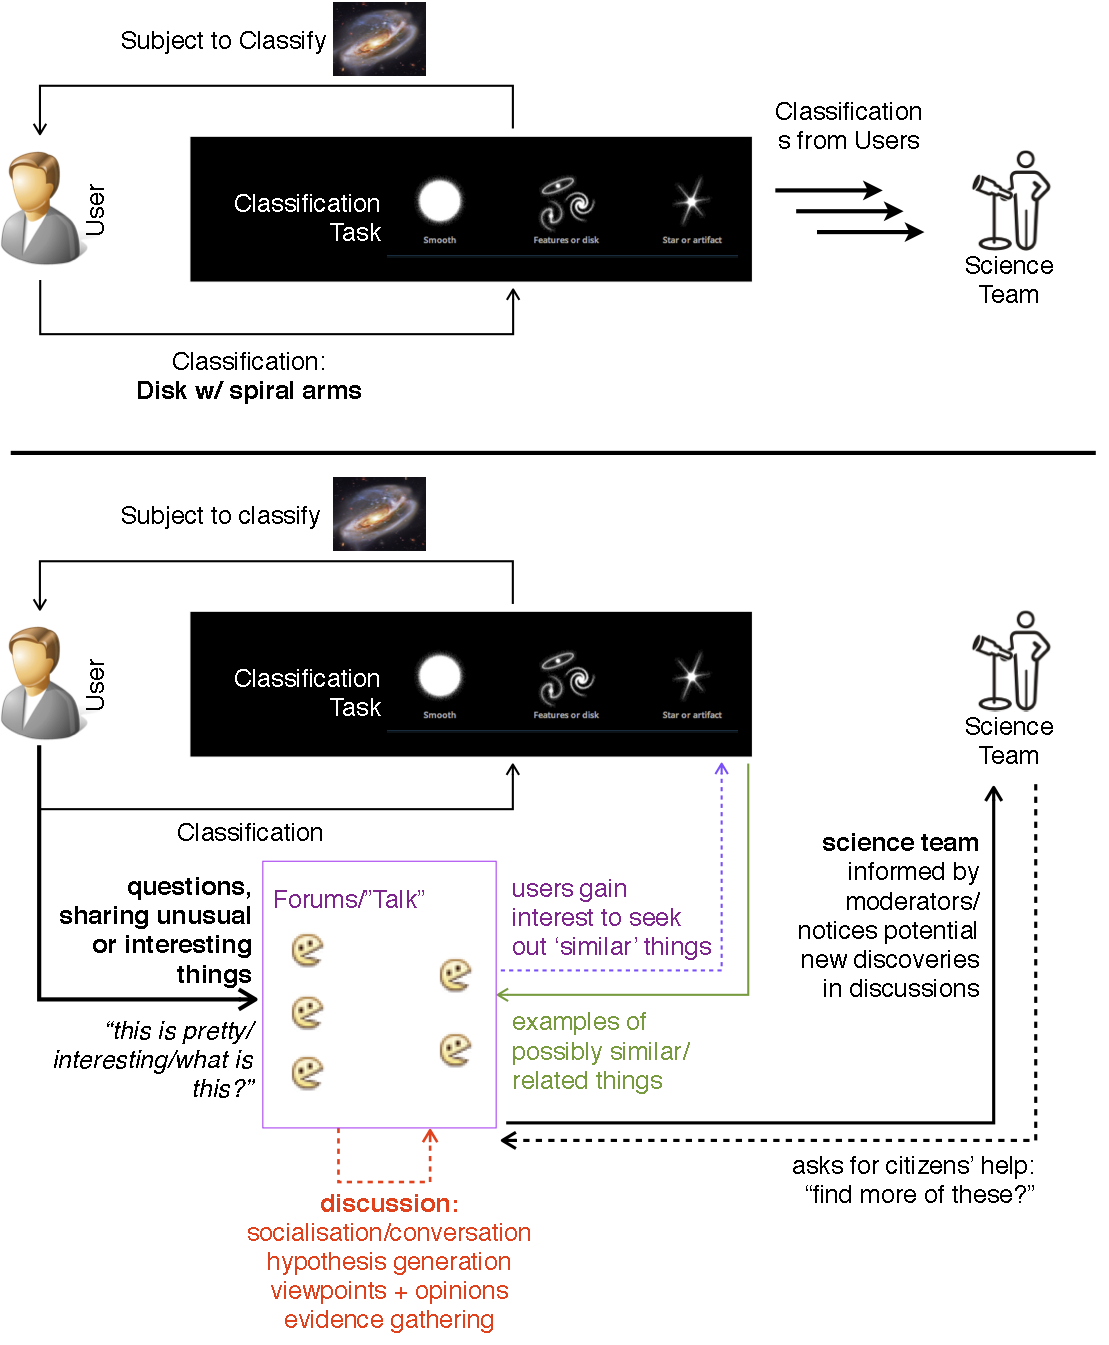
\includegraphics[width=0.44\textwidth]{imgs/twopaths.png}
\caption{\emph{Two paths to science} - In addition to the ``standard'' path (top) typical of human computation systems, where research questions are answered using annotations created by executing tasks, a second path, that of \emph{citizen-initiated serendipitous discovery} is illustrated on the bottom.  In this path, citizens initiate the process by pointing out or asking questions about subjects, spawning collaborative hypothesis generation in the discussion forums. Science teams, picking up on these discussion threads, then either perform a further investigation on their own, or start a collaborative investigation with the volunteers.}
\label{fig:twopaths}
\end{figure}

The most discussed theme was that of citizen-led discoveries, an area not originally anticipated by neither the Zooniverse nor science teams.  The original workflow intended of the Zooniverse, was the derivation of results via the set of tasks selected by the science team, which were devised to investigate a pre-selected set of problems.  This workflow, the conventional path of most human computation systems, is illustrated by the `top path' of Figure \ref{fig:twopaths}, successfully yielded a majority of the findings for Zooniverse, such as as deriving a morphological classification of galaxies (e.g. \cite{fortson2011galaxy}).   

However, the addition of discussion facilities opened a second pathway, which became apparent under a month after the Galaxy Zoo Forum first launched, when the citizen participant responsible for finding the ``Voorwerp'' posted her message that would ultimately mark the project's first citizen-initiated discovery.  This second, serendipitous ``path to science'', illustrated in the bottom path of Figure \ref{fig:twopaths}, meant that scientific questions that had not been anticipated might be identified and investigated by citizens themselves with various degrees of autonomy from the science teams.

Here, we first briefly describe the most notable citizen-initiated investigations in order to highlight the ways that citizens contributed to each.  Central to each of these were Zooniverse's facilities for collaborative discussion, which provided both the conduit and  context for users to ask questions, generate hypotheses, and even validate each others' hypotheses.  Thus, we then focus on the design of the discussion forums, and how these were refined by the team to support more effective citizen-led investigation. 

\subsubsection{Roles Assumed by Citizens in Serendipitous Discoveries}

\begin{table*}
\begin{center}
\begin{tabular}{p{1.5cm}p{0.7cm}p{1.0cm}p{10cm}p{0.19cm}p{0.19cm}p{0.19cm}p{0.19cm}p{0.88cm}}
Investigation & Date & Project & Description & CI & CH & CC & CV & Details\\
\hline
\emph{Hanny's Voorwerp} & Aug 2007 & Galaxy Zoo 
   & User `Hanny' identified an unusual object near a Galaxy in a subject; science team followed up and it remains an object of active astrophysical research.
   & y & n & n & n & \cite{lintott2009galaxy} \\
\hline
\emph{Green Pea Galaxies} & July 2007-Aug 2008 & Galaxy Zoo 
   & User `Hanny' commented on the existence of small, spherical, green galaxies that looked like peas; together with others, a group (self-named ``Peas Corp'') initiated an effort to find similar galaxies.  After a year, a science member determined that
   they represented a previously unknown class of galaxies.
   & y & y & y & n & \cite{story-of-the-peas,cardamone2009galaxy} \\
\hline
\emph{Convict Worm} & Sept 2012 & Seafloor Explorer 
   &  User `illmarinen' posted a question enquiring about an animal which he was unable to identify; a member of the science team, stated she thought this could be a new speices of worm, which she nicknamed a `convict worm', calling upon citizens to find similar specimens.  This resulted in a small number of users commenting on such subjects with the hashtag “\#convict-worm,” allowing scientists to easily collate examples and examine them together.
   & y & n & y & n & none yet \\
\hline
\emph{Kepler 16B} & May 2011 & Planet Hunters 
   &  User ``kianjin" identified a possible eclipsing binary star with a third body, later confirmed by the science team to be a circumbinary system. User ``robert gagliano" identified another potential circumbinary system, and ``kianjin'' validated it using his own models.  Upon completing these models, he contacted the science team with his analysis, who confirmed it with further analysis. 
   & y & y & n & y & \cite{schwamb2013planet} \\
\hline
\end{tabular}
\caption{\emph{Citizen-led serendipitous investigations} - A selection of investigations started by actions of citizen volunteers, 3 of which resulted in confirmed discoveries (cited in the last column above). \emph{CI - citizen-initiated}: citizens initially brought attention to the first observations relating to the discovery; \emph{CH - citizen hypothesized}: citizen participants generated the hypotheses explaining the observation; \emph{CC - citizen evidence collecting}: citizens coordinated efforts to find more evidence; \emph{CV - citizen validated} - citizens built models to validate/confirm hypotheses.}
\label{tbl:serendipity}
\normalsize
\end{center}
\end{table*}

To better understand the process of citizen-initiated discovery, we consulted with the Zooniverse team to identify a set of examples to analyse, that started with citizens and resulted in a findings verified by the science team.  While this method may have overlooked citizen-initiated investigations among the multitudes of posts, our goal was first to understand how discoveries were initiated and unfolded when they did occur.  From the proposed set, four were selected that reflected a variety of citizen roles, summarised in Table \ref{tbl:serendipity}. For each example, we assembled all available written evidence for each, including discussion and talk posts, notes made by the science team, blog posts by the science team, and even a few blog posts by citizen participants.  These were then analysed to identify the kinds of roles assumed by various citizens during each process and the resulting workflow.

All four began with a user calling attention to something they encountered during a task, although the purpose for making these posts varied; in two (Voorwerp and Convict Worm), the user was merely asking for help identifying an unknown object they saw.  With the Peas discovery, meanwhile, the intention at the beginning was primarily social, commenting that she found things that ``looked like peas''.  In the Kepler findings, by comparison, the citizens already had a hypothesis about what they had found, and had conducted a partial analysis prior to first posting.

The degree of further citizen involvement also varied among the four examples. For the Voorwerp discovery, the science team took over the investigation shortly after the citizen pointed it out. In the other examples, however, there was more autonomous action by citizens; in the Peas case, for example, citizens self-organised a collection of samples and an informal analysis for approximately a year before the science team caught notice and took significant interest in their findings.  (The so called self-organised ``pea hunters'' even called themselves the  ``Peas Corps'' \cite{story-of-the-peas}).  In convict worm case, meanwhile, the science team intervened early, and then immediately solicited help from to identify similar subjects.  This was done because the team did not know whether this was a one-off worm or common enough to constitute a distinct species. Finally, with the Kepler discovery, as previously mentioned, the users conducted an entire hypothesis validation process, consisting of modelling and light curve analysis, using their own sets of tools.

\subsubsection{Analysis of Cases}

The variations in outcomes among these cases reflect several underlying differences among the situations, shaped by a common set of constraints.  One such constraint pertains to science team time and attention; due to the rate at which discussions occured (typically hundreds of posts a day), it was generally not feasible for them (usually comprised of 2-4 busy individuals) to monitor all discussions for possible serendipitous leads.  A core role of moderators, thus, was to filter and signal potential findings to the science team.  Yet, in a significant number of cases, this is difficult for moderators to ascertain, as, being citizens themselves, they had access to the same resources as normal volunteers. The result was that moderators would have to make a best guess about what to flag, resulting in the possibility of overreporting (which overwhelmed science teams) or underreporting (which may miss possible leads).  The second constraint, thus pertains to access to tools, data sources and expertise. 

Highlighting these constraints and how they influenced the cases above, the \emph{Voorwerp} discovery process unfolded as it did because, being a rare astrophysical body quite unlike others, it quickly popped out to scientists soon after it was discovered.  In this case, due to lack of access to other data sources or expertise, there was little that other citizens could contribute; moreover, being such an unusual form, and most others had never seen anything like it. To perform the investigation, the science team cross-referenced databases and tools that volunteers didn't have access to, running their own analyses before eventually scheduling time on a deep-space telescopes with colleagues to gather more data.  The \emph{Peas} scenario, meanwhile, worked quite quite differently.  While not common, pea galaxies were seen regularly enough that they were recognized by other citizens, which sparked the ``pea hunt'' movement. Meanwhile, it was in this case that the science team, with limited time, paid little attention to the galaxies for a while, according to a science team member because they were particularly busy processing data being generated through the ``main path'', but also partially because it was believed the greenish appearance of the peas was merely artefactual of the imaging apparatus, as ``green glitches'' were quite common in the images. 

The Kepler example stands out from the rest in that the citizens essentially derived their own astronomical models generated from light curves autonomously without science team intervention.  Although the two users declined to identify their backgrounds, it was clear from their responses and modelling capabilities that they possessed extensive knowledge of astrophysics. Having expert users as in this example highlighted to the Zooniverse and science teams citizen volunteers could be true collaborators, and that citizen science systems served another important purpose, which was to bring experts together around common problems of interest, across traditional organisational, national and cultural boundaries.

% \subsubsection{Individual Citizen-Initiated Discovery: \emph{Hanny's Voorwerp}}
% In August of 2007, on the Galaxy Zoo forum, the user ``Hanny'', spotted an usual blue-shaped object in a subject beneath a galaxy, and posted a question in the Galaxy Zoo forum. Within an hour, two separate members of the science team had shown an interest in the subject and attempted to identify the shape, continuing to comment for a further thirteen days, concluding it was something ``weird [...] I'd like to know what it is''.  Within a few months, the science team confirmed  it as a phenomenon of unknown origin unlike any other previously observed, and remains an object of active astrophysical research today \cite{lintott2009galaxy}.

% \subsubsection{Individual Citizen-Initiated Discovery: \emph{Hanny's Voorwerp}}
% In August of 2007, on the Galaxy Zoo forum, the user ``Hanny'', spotted an usual blue-shaped object in a subject beneath a galaxy, and posted a question in the Galaxy Zoo forum. Within an hour, two separate members of the science team had shown an interest in the subject and attempted to identify the shape, continuing to comment for a further thirteen days, concluding it was something ``weird [...] I\''d like to know what it is''.  Within a few months, the science team confirmed  it as a phenomenon of unknown origin unlike any other previously observed, and remains an object of active astrophysical research today \cite{lintott2009galaxy}.

% Regarding the finding of the discovery, the object in question was not the main focus of the subject, which was in fact a galaxy located behind it. Since the classifying interface essentially only allowed her to mark the galaxy, she turned to the forum to ask her question.  Without the forum, being available for her to easily post a question, it is possible that Hanny may have not done anything, and the object may have gone undiscovered. %

% % Neal's original >>
% % In August of 2007, on the Galaxy Zoo forum, Hanny van Arkel, a Dutch school teacher who identified herself as user ``Hanny'', spotted an usual blue-shaped object in a subject beneath a galaxy, and posted a question in the Galaxy Zoo forum. Within an hour, two separate members of the science team had shown an interest in the subject and attempted to identify the shape, continuing to comment for a further thirteen days, concluding it was something ``weird [...] I\''d like to know what it is''. Thereafter, discussion on the thread stalled until December 2007, when Hanny asked about whether the mystery had yet been solved. The science team then redoubled their efforts to identify the shapes. After scientists made the thread more prominent, other Galaxy Zoo users began to post examples of other subjects, as well as collections of data, in order to help identify the shape. 

% % The object in question was not the main focus of the subject, which was in fact a galaxy located in the centre of the image. Since the classifying interface essentially only allowed her to mark the galaxy in the image, without the forum thread drawing attention to the oddity present, it is possible that it would have gone unnoticed. Hanny's thread did not result in significant contributions from users, but it was instrumental in drawing the attention of scientists to the object, allowing them to carry out further tests and analyses that users could not - Requesting for telescopes to be pointed at the object, for example. As a result, the discovery relied heavily on the science team but could not have taken place without the actions of an individual citizen. A more detailed chronicle of Hanny's discovery was documented by Lintott et al \cite{lintott2009galaxy}.
% %http://www.galaxyzooforum.org/index.php?topic=3802.0

% \subsubsection{Group-Led Discovery: \emph{Galaxy Peas}}
% In July of 2007, the user ``Hanny" created a post on the Galaxy Zoo forums entitled ``Give Peas a Chance". The post contained images showing small, spherical, green galaxies, which according to Hanny looked like peas. This post was intended as a joke, but the peas captured the imagination of Galaxy Zoo users and the thread grew, with more and more users creating posts containing such galaxies. A group calling itself the ``Peas Corp" went in search of further peas within the Galaxy Zoo subjects and created several collections of subjects. After almost a year, the science team noticed common characteristics shared by these peas, resulting in a call to action from science team member ccardamone, known as the ``peas project", intended to gather peas with certain properties. 

% As a result of the peas project, users found and analysed various subjects to create a list for further analysis, allowing the science team to carry out tests to identify what `peas' are. This collaboration between the science team and the Galaxy Zoo user base resulted in a discovery which may have gone undiscovered otherwise.

% ORIGINAL -
% Due to the method used to capture the images used for Galaxy Zoo, subjects could appear in a variety of colours which did not reflect their colours in the visible spectrum. This resulted in objects appearing in subjects as green, when they were, in fact, blue. These green objects were particularly interesting to Galaxy Zoo users, who perceived green to be a strange colour for a galaxy.  The majority of such subjects simply included camera glitches, which had resulted in light only being absorbed in one filter, giving objects a green appearance. However, certain objects were not glitches and appeared as small, tight, green spheres. Users used the term “peas” to refer to the objects in question, after a joke thread started by ``Hanny'' (the same user as the previously mentioned discovery) on the Galaxy Zoo forums, `Give Peas a Chance,' in July of 2007. The strange colour and shape of these galaxies captured the imagination of many galaxy zoo users, who formed a group called the `Peas Corp' and went in search of subjects containing peas, creating various forum threads to collect them. While the science team were particularly busy in the early months, the collections of peas eventually drew their attention a year later in July of 2008 and they discovered that these galaxies shared  certain interesting features, including specific red shift values and bright spectral lines caused by double ionised oxygen particles (OIII). This resulted in a `call for action' from the user ccardamone (a member of the science team) known as the `peas project', which requested subjects containing peas with certain properties.

% As a result of the peas project, users found and analysed various subjects in order to create a suitable list for further analysis. This allowed the science team to carry out various tests and statistical analyses on the objects, to attempt to explain the strange appearance of these particular objects and to identify what `peas' are. This collaboration between the science team and the Galaxy Zoo user base resulted in a discovery which both sides may have missed otherwise: Users noticed the objects were strange, but did not realise their significance, while the science team were able to identify the significance, but may not have identified `pea' galaxies as a specific class of galaxy, without the actions of the user base.


% http://www.galaxyzooforum.org/index.php?topic=3638.0 and http://www.galaxyzooforum.org/index.php?topic=270633.0
%comment from markus: consider adding the 'offline' communication stream here which happens when scientists start to discuss forum observations by mail for example. Is it possible to detect that something happened 'offline' by simply looking at what is visible online? How is the information flow between 'online' and 'offline' discourse? Are there specific actors delivering information into the one or the other direction? What about all other people which are not involved 'offline'? Do they know about this 'hidden' activity? Does it motivate or demotivate people when something is going on without them? Are all users equal in this regard?

% Hanny's Voorwerp is the clearest example of this - Evidently work is going on 'behind the scenes', but this doesn't seem to put users off - They don't seem to understand why they aren't allowed to know about things, but they do seem to wait somewhat patiently for the 'reveal' of information. However, it's quite possible comments which were more negative have been deleted or edited in the meantime and there's no way of knowing what was said by whom to whom outside of Zooniverse. Besides which, we can only tell that there's hidden activity when it's made somewhat clear - Which would be the same situation for users. Truly hidden activity would be just as hidden to us, at least from looking at the forums. In that particular case, the actors are Hanny and the science team - Moderators actively admit to not knowing anything.

% \subsubsection{Asking for Help on a Possible Discovery: \emph{Convict Worm}}
% In August (Potentially September) of 2012, the user `illmarinen' made a comment on the talk page for a Seafloor Explorer subject, asking about an animal which was present in the image which he was unable to identify. A member of the science team responded, stating that she thought this could be a new discovery, which he nicknamed a `convict worm', adding that he was actively seeking subjects where the worm was present. This resulted in a small number of users commenting on such subjects with the hashtag “convict-worm,” allowing scientists to easily collect examples of the potential new species. A blog post published shortly after the discovery encouraging users to tag convict worms has led to sustained and frequent tagging of subjects perceived to contain the worms, allowing suitable subjects to be gathered without requiring changes to the classifying interface, which did not allow flagging of convict worms.
% %(http://talk.seafloorexplorer.org/discussions/DSF1002n2b?object\_id=ASF00009jp)

% \subsubsection{In-Depth Citizen-driven Investigation: \emph{Kepler 16B}}
% In May of 2011, Planet Hunters user Kian Jek made a comment on the Planet Hunters Talk website under the username ``kianjin", sharing a subject which appeared to show an eclipsing binary star with a third body present. A research team led by Slawson had already began analysing the system in question and it was eventually discovered that this system was a circumbinary system - A system in which a planet orbits two stars simultaneously. 

% After the announcement of this discovery, named Kepler-16b, Meg Schwamb of the Planet Hunters science team published talk pages with links to all known eclipsing binaries present in the Planet Hunters data. In February of 2012, the user Robert Gagliano, using the username ``robert gagliano", searched through each of these subjects for signs of potential planets and noted two transit features (reductions in light intensity caused by a body `transiting' between the star and the satellite) present in the subject SPH10052872. Kian Jek later predicted and confirmed a third transit and was then able to create models and graphs to better understand the lightcurves. Upon completing these models, Jek had confirmed to the best of his abilities that SPH10052872 showed a circumbinary planet and at this point, contacted the science team, who would be able to carry out further analysis which he could not. 

% While Gagliano and Jek required the intervention of the science team to confirm their discovery, their research was much more in-depth than in the other examples shown. Additionally, through their work, they had proven that something of interest was present and had successfully identified the item to the best of their abilities: They were not asking ``what is this," but rather, they were asking for confirmation of their theories. 

% ORIGINAL -
% In May of 2011, Planet Hunters user Kian Jek made a comment on the Planet Hunters Talk website under the username ``kianjin", sharing a subject which appeared to show an eclipsing binary star with a third body present. A research team led by Slawson had already began analysing the system in question and it was eventually discovered that this system was a circumbinary system - A system in which a planet orbits two stars simultaneously. 

% After the announcement of this discovery, named Kepler-16b, Meg Schwamb of the Planet Hunters science team published talk pages with links to all known eclipsing binaries present in the Planet Hunters data. In February of 2012, the user Robert Gagliano, using the username ``robert gagliano", searched through each of these subjects for signs of potential planets and noted two transit features (reductions in light intensity caused by a body `transiting' between the star and the satellite) present in the subject SPH10052872. Kian Jek later predicted and confirmed a third transit and was then able to create models and graphs to better understand the lightcurves. Upon completing these models, Jek had confirmed to the best of his abilities that SPH10052872 showed a circumbinary planet and at this point, contacted the science team, who would be able to carry out further analysis which he could not. 

% While Gagliano and Jek required the intervention of the science team to confirm their discovery, their research was much more in-depth than in the other examples shown. Additionally, through their work, they had proven that something of interest was present and had successfully identified the item to the best of their abilities: They were not asking ``what is this," but rather, they were asking for confirmation of their theories. 

\subsubsection{Problems Observed in Expanding Discussion Forums}

%  original from Chris/Rob, turned into below
% It was designed to enable links to be made easily between classification and discussion and to allow science team members as well as advanced volunteers to quickly notice when users were talking about discoveries of potential interest. To understand the design drivers for talk's system of object-orientated discussion, consider the case of a new classifier who had spotted a `pea' in a Galaxy Zoo image. Even if they were to move to the forum, they would have been unable to search for discussion of their or similar objects unless they made the same mental leap to think of a small round celestial object as a kind of vegetable. If they found the right thread, they would have had to upload their image to a linear 	discussion which might well be in the middle of more detailed analysis. In Talk, by contrast, a single click after classification invites discussion, and lands on a page dedicated to discussing the object that's just been classified. Our putative pea-finder would immediately be able to see what had already been said about this system, and - were it already to be tagged as a 'pea' - to click on 'pea' and realize that there was a much broader conversation going on. This model has been broadly successful, with most of the discoveries made by the Planet Hunters project (including PH1b, the first planet in a system with four stars) coming from discussion between users who found interesting things in the interface and a community of more advanced workers who were able to help the science team follow-up on those discoveries. 

% ``number of emails received by the team'' -> what kind of emails? and how did this prompt use of a forum
%% Michael Nielsen's book > on networked science --- Reinventing discovery
%% http://press.princeton.edu/titles/9517.html

% Rob's original >> 
% Beyond achieving the goals set out to reduce this support burden, users made use of the site to identify, discuss and advocate for serendipitous discoveries. The canonical example is the object now known as Hanny's Voorwerp \cite{voorwerp}, a galaxy-scale glowing gas cloud which turned out to have been ionized by activity associated with neighboring galaxy's rapidly feeding black hole. In this case the discovery was reported on the forum, but the follow-up work was carried out by the science team themselves. In other examples, though, much more sophisticated behaviour was seen. The discovery of the Galaxy Zoo Peas \cite{Peas}, for example, saw a group of volunteers who had identified the presence of small, round and green objects (hence the name) in the background of some images work together to download and explore metadata on these objects, to write database queries and even, eventually, to create their own citizen science site to assist in further classification of these intriguing objects. The peas turned out to be a new class of galaxy, the most efficient stellar factories in the local Universe, and remain the subject of vigorous debate in the professional astronomical community.  The process by which the Galaxy Zoo science team picked up on the participants' posts in the Discussion forums about ``green peas'' and ended up with a significant new discovery is documented in detail on the Zooniverse Blog\cite{story-of-the-peas}.

%% specious stuff emax wrote, please check 

Over the course of the Zooniverse project, the role of the discussion forums came to serve several important functions for project success, including providing a space for peer question-answering support, serendipitous collaboration, and social community building and sharing. However, as the forums expanded, it became clear that aspects of the design of the original forums impeded their effective use.   

First, standard, linear message-board format of the Galaxy Zoo Forums became difficult to navigate as the size of these forums grew.  As boards expanded, moderators struggled to keep boards thematically consistent, and threads often ended up in different boards, were duplicated, or blended themes.  When this occurred, it became difficult for users (especially new forum visitors) to either find a place to post a question, or see if the answer already existed, and struggled to find relevant threads across boards.  The result was that new users with questions often resorting to simply creating new threads or tacking a post on the end of a recent, irrelevant thread.  Such problems, including fragmentation and duplicity mirror those well-known  in many other large, online threaded discussion boards (e.g., \cite{murphy2004graduate}), and posed a serious challenge as some GalaxyZoo boards expanded to over 5000 threads, collectively comprising over 650,000 posts. 
After several of the serendipitous discoveries were made, other problems pertaining to the lack of integration between the forums and tasks became apparent.  The forums, which were built using a general-purpose open-source online discussion system\footnote{Simple Machines - \url{http://www.simplemachines.org/}} lacked any sort of Zooniverse domain-specific notions such as of subjects, task or object types. This meant that posts about the same subject could not be easily viewed, nor could posts about classified objects of like or similar types.  Keywords search facilities could be used to a limited extent, but also yielded very voluminous and noisy results. This meant that steps critical to the second pathway to discovery described earlier, as well as along the to peer-supported question answering were made difficult by forum organisation.

% that each, itself, contained a set of message threads.  Each message thread, in turn, consisted of a linear sequence of posts; posts to a board either started a new thread, or were appended on the end of an existing thread.  Several drawbacks of this model became apparent as the board grew; first, threads on the same topic might appear in different boards.  Second, multiple threads on the same topic could appear within a board, which became increasingly an issue as the number of threads per board increased, and users found it increasingly difficult to identify relevant threads before creating a new one. (The main GalaxyZoo forum has several boards each with over 5000 threads that make up more than 100k posts, making navigation and retrospective analysis very daunting.)  Finally, since posts were strictly linked to a single thread, it was difficult for insights to be gathered on topics across threads; in particular, discussions about particular topics, such as types of celestial bodies, similar objects, artefacts, and phenomena would become fragmented among threads.  As threads grew in length (in discussions), topics often diverged from the topic of the top post, meaning it was difficult for users to anticipate the contents of a thread by looking at the thread's title.  

%Given these forum limitations, it became the role of the forum moderators to monitor and de-fragment threads as necessary, moving posts between threads and even boards.  After trying to act as moderators themselves, the science team appointed a selection of the most active citizen participants with moderator privileges and status in the system.  But despite the dedication of this new group of volunteers, this proved often a challenging task as participation in the forums grew; the result was that regular members often posted messages to moderators to help them out, pointing out threads to merge and posts that would best fit elsewhere.

%While this technique succeeded at the beginning, overall participation among new users (across all Zooniverse projects) leveled off after an initial period of growth, and many factors suggested that the difficulty of navigating the forums was responsible. Such low adoption rates among new users were seen across projects, although a small set of core contributors seemed to continue to use it regularly.  (In fact, this core community also resisted any attempts to modernise and migrate discussions to a more structured format, which we describe next).

 % and still is the mechanism by which the original Zooniverse forums operate today, primarily among a small set of core contributors.  overall participation levels in the forums levelled off after an initial period of fast growth. Such low participation rates were present across Zooniverse projects such as Moon Zoo and Old Weather, and messages suggested that it was the difficulty of navigating these forums that was its cause.  cross the boards, however, it is worth noting that a core community continued to use the forums with a space to discuss the historical aspects of the project, in particular.

%% key affordance: linking between subject and its discussion, and then horziontally allowing tagging as a mechanism of allowing similar posts to be identified

\subsubsection{Integrating Discussion to Support Citizen-Led Workflows}

In response to these problems, the Zooniverse team decided to implement a bespoke discussion tool that would integrate into the tasks and facilitate discussion around subjects and objects. Their new system, called \emph{Talk} was introduced with Planet Hunters in 2010, and rolled out to all subsequent launched projects.  

Talk offered several unique features; first, every subject had a unique \emph{talk page}, corresponding approximately to a thread where discussions about that particular subject could be centralized.  Talk pages were thus indexed (identified) by subject.  To support simple cross-referencing, Talk identified when the name or identifier of a particular subject was mentioned, and replaced the mention to the talk page of that subject.  Second, the team added tagging support, so that tags added to a post could be easily collated with other Talk pages with the same tag. This was done based on insights from the \emph{Peas} discovery, in which there was a need to be able to collect posts about ``green objects'' and ``objects that look like peas''.  After the launch of Talk, this feature proved useful in the ``Convict worm'' case described earlier, dramatically simplifying the process of collating posts about the possible new species.  

A side effect of the new tagging features was that users were made aware of active citizen-led investigations that were underway simply through the trending tag display.  This could be used to recruit the attention of citizen towards active problem solving efforts, such as the identification of convict worms in new datasets.

\subsubsection{Encouraging Discussion and Avoiding Thread Death}
%% TODO quant: any statitstics on discussion rate? 
	
%Based on the discoveries described earlier, the science team began to perceive the tasks as serving a secondary important function beyond providing the labels and classifications as designed; namely, to serve as entry points to discussion, and show participants things they might want to discuss or talk about.   %In particular, this second function produces science through the intervention of `superusers' who may not classify themselves but who are able to make use of and further analyze interesting discoveries. observed that many of the comments provided some degree of insight and were useful when identifying unusual features of subjects.  

Despite the growth of the forums, only a small percentage of users who performed tasks ever visited the discussion forums, and that those who participated in the forums were predominantly regular users. Thus, to attract more diverse perspectives, the team sought to increase the proportion of volunteers who participated in the forums.  To do this, the team sought to \emph{reduce the barrier of execution} of discussion, that is to make it easy to enter a discussion on a particular subject or topic, and to make the discussion facilities more salient\cite{norman2002design}.  

These goals were realised with \emph{Talk} in several ways; the first was by prompting users explicitly  'Would you like to discuss this?' after each task.  While this posed the risk of adding the extra burden of dismissing these prompts when a discussion was not desired, no effect was seen on long-term interactions.  For other projects, the team merely made a salient ``discuss this'' button which appeared on a subject after it was classified.  While the strategies differed slightly in effect, the resulting difference, in number of discussions started per subject, was not significant.  The team is currently testing variations of these designs, which will be reported in a later analysis.

A second problem pertained to \emph{authority thread death}, in which a voice of perceived authority, usually a moderator, responding to a thread causes it to fall silent.  The  explanations for this phenomenon have been proposed in terms of social actor theory,  reciprocity and social network theory \cite{preece2003online}, and incorporate factors such as people not wishing to be seen to be challenging authority, to there being a diminished need.  To compensate for this phenomenon, the Talk design team decided to put a ``twitter-like'' 140-character text box underneath each subject, to encourage participants to make quick comments on the subject with whatever they liked.  This format, being less structured, formal, and more egalitarian than the forums, meant that people would only see a selection of recent ``tweets'' about the subject beneath theirs, and would be less likely to be put off by a moderator's input.  This facility significantly increased comments made about subjects; and the team is currently pursuing potential strategies to process  derive insights from these comment streams.

% The status of each user, specifically whether or not they were a moderator or member of the science team, was also suppressed to reduce this effect.  %  AND THI%
% Although killing threads seems to rarely be an actual intention of any of the Galaxy Zoo Forum moderators, as exhibited by their occasional efforts to try to revive these threads by asking rhetorical questions to seldom avail, this problem nonetheless occurred frequently in the original forum.

%The second version of Talk sought to circumvent thread death by simply adding an additional affordance for adding a comment about a subject on the Talk page.  Taking inspiration from microblogging interfaces, the team decided to put a ``twitter-like'' 140-character box underneath each subject, to encourage participants to comment on the subject with whatever they liked.  This format, being less structured, formal, and more egalitarian than the forums, meant that people would only see a selection of recent ``tweets'' about the subject beneath theirs, and would be less likely to be put off by a moderator's input.  The status of each user, specifically whether or not they were a moderator or member of the science team, was also suppressed to reduce this effect.  %  AND THIS WORKED TODO 

%% TODO someone: 
%% The effect of the introduction of this Twitter is ___________________________

%% todo this dies:: 
% \subsubsection{Active Collaboration with the Science Team}
% Structured collaboration also proved effective. Galaxy Zoo science team member Bill Keel from the University of Alabama was able to spend time on the forum, and asked for help with searches for objects such as galaxies which appear to overlap \cite{overlap} (distant galaxies used to illuminate foreground ones can be used to probe the dust content of systems, a matter of some importance to astronomers). This work was also successful, but required Keel to spend substantial time as part of the forum community, something that other science team members were unwilling or unable to do. 

%% DOTO SOMETHING ELSE ABOUT COLLABORATION HERE?
%(This was perceived as not the only problem with the Forums and led to the design of the Talk forums, which anchored discussions around subjects, and reduced the need for a person, a role fulfilled Bill Keel to coordinate discussions about the same subjects or topics. and to make those discussions visible to both the science team and the participants.) Furthermore, by 2009 the forum had become less popular; the percentage of Galaxy Zoo users posting on what was a standard \emph{Simple Machines forum}\footnote{} was very low (less than two percent) and with more than 500,000 posts in more than 10,000 topics it had become difficult to navigate. While it still served the need of a core constituency, it was not engaging the majority of Galaxy Zoo classifiers in science. 

\subsection{Dimensions of Engagement}

The second theme pertained to factors that drive user motivation and sustained engagement. Here, we describe the key experiences these have impacted the design of Zooniverse projects over time.

\subsubsection{A Landscape of Interestingness, Speed, and Reward} 
Over the course of different projects, some projects experienced more immediate uptake and sustained higher participation rates than others.  The team has been seeking to understand the factors that may be responsible for this variability, in order that they might be made more predictable and controlled.  The team engaged in a qualitative analysis, starting with a large range of potential factors ranging from the design of the tasks, to launch strategies, to the types, sources and properties of subjects being examined. 

This analysis, relying on evidence from multiple sources, including discussion forums, talk pages, and time-based per project performance profiles, found the strongest support for three factors:\emph{interesting-ness of subject}, \emph{difficulty of task}, and related to these two, the \emph{frequency and form of implicit reward}. Other factors, such as type of task, domain of origin, worthiness of cause (e.g., cancer research or deep space research), and source of data, did not generate conclusive findings, except subject media type, which we discuss later.

The first factor, \emph{interesting-ness} is difficult to characterise, as different users found interest in many different things in different ways.  However, beyond the general interest in science that drives most Zooniverse participation, certain types of subjects carry much more engagement.  These subject seem to carry aesthetic or emotional value, such as ``beautiful and mysterious'' photos of deep space, or the ``cute''candid photos of animals of Snapshot Serengeti.  Sometimes, it is the interestingness of the task in the context of the subject, such as the ship logs of Old Weather, described as ``like deciphering an unknown history''.  Subjects in such categories seem to continuously generate the dedicated attention of followers.  Several forum posters have commented on the addictive nature of all three of these projects; the line of denial ``I'm not addicted to Snapshot Serengeti'' becoming a meme in both its forums and on Twitter.

Interesting subjects worked best if they appeared frequently enough while performing tasks, and tasks involved enough variability from one classification to the next.  If tasks involved long stretches of nearly identical subjects, such as was the case in a potential pilot of a project involving finding seals on aerial glacier photos, users tended to get bored quickly. The team explained this using the theory of \emph{implicit reward} \cite{implicitreward}; in the absence of other external reward, the subject delivered on successive tasks served implicitly as a reward for participating. Thus, when new tasks involved classifying subjects that were occasionally beautiful or interesting, participants were stimulated to continue. %.  Since Zooniverse intentionally provided no \emph{skip} facility, viewing more subjects required completing more tasks.

To reduce the likelihood of long stretches of monotonous subjects in real datasets, more recent projects added a task scheduling strategy, that involved quickly isolating subjects which contained potentially interesting objects (using the classification actions by users), and to add these to the task queues of other users who might be suffering from a monotony of unvarying subjects, as indicated by identical or ``nothing here'' classifications.  In Worm Watch Lab, for example, an algorithm was devised that would take subjects that were classified by at least one user to contain egg-laying events, and scheduled these into the queues of users who had not witnessed egg-laying events in their most recent classifications.  User feedback was positive, and this algorithm was re-extended to other projects such as Milky Way's Bubbles. 

%re-represented these to users who  a result, the system could present users with such subjects on a regular basis, to prevent users being forced to identify large numbers of subjects without seeing an egg-laying event

%% piloting a domain --milky way bubbles and Clouds
% In a number of projects th
% In the first launch of YYY, participation dropped off because the frequency of reward was simply too low; a participant could be made to look at more than 1000 blank subjects before coming across one that contained a Galaxy.  In order to compensate for this, more recent projects attempt to quickly identify subjects which contain an object of interest and those which do not, to prevent users becoming bored or disillusioned with the classifications tasks. In Worm Watch Lab, for example, the science team were unaware of which subjects contained footage of worms laying eggs and which did not. To overcome this, the system assumed that subjects which were classified as containing egg-laying events by three or more users were highly likely to contain such events. As a result, the system could present users with such subjects on a regular basis, to prevent users being forced to identify large numbers of subjects without seeing an egg-laying event. 

%% While the Zooniverse team are currently developing a framework for doing \emph{in situ} quantitative analysis , derive quantitative measurements of specific interface affordances, the

%% engagement
%%   status ::
%%   questions answered in the forums they leave
%%   thread death

However, even monotonous sequences of subjects sustained participation if they were \emph{could be performed quickly}. The team's interpretation of the resilience of user boredom for quick tasks was that such tasks provided a different kind of implicit reward feedback, pertaining to the feeling of accrued accomplishment, that is, finishing tasks quickly spurred sustained participation.  This effect was observed in Moon Zoo, where users were  keen to keep classifying thousands of photos of boulders in photos of the moon, despite their similar, monotonous appearaence, with little hope of variation.  This task was generally very quick to perform due to its simplicity and efficiency of interface. Participants also performed an average of $MMM$ classifications of Moon Zoo, compared to $YYY$ comparable tasks, for example in ZZZ, a substantially more difficult project.

% TODO:
% Galaxy Zoo Craters vs Milky Way Project Bubbles - Essentially same task, but Bubbles much more complex due to arc tools - fill in MMM, YYY and ZZZ above with figures from these projects. Note that from March 8th 2012, the Milky Way Project changed to only include subjects which were guaranteed to contain a bubble - seemingly, no change has been made to the interface itself.

% By comparison, there was no perceived preference in research field, topic, or task type, and substantial variability among the success rates for projects existed within each of these categories.  For example, astronomy projects such as XX maintained attention and engagement, while YY, also from the same field and of essentially the same task type, levelled off in participation after an initial period of enthusiasm.   Furthermore, it was deemed that tasks of one particular type, such as classifying tasks, were not significantly more successful than transcription, given the success of projects like \emph{Old Weather} and \emph{Notes from Nature}, although the very different nature of these tasks makes direct comparison difficult.

% that appealed to the general audience, and it was these projects that exhibited the greatest user retention as well as attracted the most users.  In particular, Galaxy Zoo, which features a large number of beautiful photos of galaxies and deep space, and Snapshot Serengeti, which features an abundance of ``candid'' photos of popular animals in the wild were each 

% \begin{table*}
% \begin{center}
% \small
% \begin{tabular}{llp{1.4cm}p{1.2cm}p{1.4cm}p{2.5cm}}
% \hline
% Project & Classifications & Talk items & Avg talk per classif. & Talk items per Subject & Talk workflow \\
% \hline
% \hline
% %Ancient Lives & ??? & ??? & ??? & ad hoc & ??? & ??? & & ad hoc \\
% %Andromeda Project & 1,091,406 & ??? & ??? & & prompted  \\
% Cyclone Center & 218,317 & 1615 & 0.7\% & & prompted \\
% Galaxy Zoo 2 & 7,907,151 & 89,956??? & 1.1\% & & prompted  \\
% Galaxy Zoo Hubble & 7,458,781 & ??? & & & prompted  \\
% %Milky Way (Bubbles) & ??? & ??? & ??? & none & ??? & ??? & & prompted \\
% %Milky Way (Clouds) & ??? & ??? & ??? & ad hoc & ??? & ??? & & ad hoc \\
% %Notes from Nature (Herbarium \& Calbug) & 209,169 ?? & - & - & none & 4,208 ?? & 2.0\% & & ad hoc \\
% %Notes from Nature (Ornithological) & ?? & - & - & none & ?? & 2.0\% & & prompted\\
% Planet Four & 3,900,785 & 32,097 & 0.8\% & & prompted \\
% Planet Hunters & 19,179,696 & 427,917 & 2.3\% & & prompted  \\
% Seafloor Explorer & 1,682,511 & 33,367 & 2\% & & prompted \\
% Snapshot Serengeti & 7,800,896 & 39,250 & 0.5\% & & prompted  \\
% Space Warps & 7,037,472 & 20,978 & 0.2\% & & ad hoc \\
% Worm Watch Lab & 90,350 & 855 & 0.9\% & & prompted  \\
% \hline
% \end{tabular}
% \caption{\emph{Favourites and Talk Items per Classification per Project} - The above table shows the number of favourited relationships and talk items in the Zooniverse database as of September 2013, for each of the above the projects.  (Only projects that used Zooniverse Talk were included to allow direct comparison, and Galaxy Zoo Forum figures were not included, which can be found directly on the forum site.) In the ``workflow'' column, ``prompted'' means users were prompted with a dialog asking whether they wished to discuss the item, while ``ad hoc'' means a button providing access to the talk page for that subject was made available in the interface for users at any point.}
% \label{tbl:favourites}
% \normalsize
% \end{center}
% \end{table*}

% time periods: Galaxy Zoo 2 (2009-02-16 - 2009-05-21), Galaxy Zoo Hubble (2010-04-17 - 2012-01-31), Planet Hunters (2010-12-15 - 2013-07-16), Cyclone Center (2012-09-27 - 2013-06-12), Andromeda Project (2012-12-04 - 2013-07-17), Snapshot Serengeti (2012-12-11 - 2013-07-17), Planet Four (2013-01-07 - 2013-07-17), Notes from Nature (2013-04-19 - 2013-07-17), Space Warps (2013-05-07 - 2013-07-17), Space Warps (2013-05-07 - 2013-07-17), Worm Watch Lab (2013-07-03 - 2013-07-17), SeaFloor Talk (13.09.2012 - 12.09.2013), SeaFloor Classification (13.09.2012 - 17.07.2013)

% Based upon popularity of the various projects and tasks, the team gained considerable insights on the tricky question of \emph{what drives people to keep coming (back)}.   
% Tasks, however that were not particularly interesting can still sustain engeagement if they are \emph{easy}

% Since Galaxy Zoo 2 there have been project-o-meters' created to show progress of the community toward a common goal or project completion. The Planet Hunters `Planetometer' displays the total number of classifications of the project, as well as the number planet candidates discovered. The `Moonometer' shows the cumulative area of the Moon that Moon Zoo has scoured for craters in various units\footnote{Units include Square Miles, Football Fields, Taj Mahals, Switzerlands, Utahs, Texas, Polands, Wales, Whales and others -- see http://www.moonzoo.org/moonometer}. These counters exist on many projects but not all.

% Where they do exist these counters do not normally appear to drive people to participate, but they do appear to be heavily discussed by people writing about projects and by dedicated users noticing the approach of milestones. In the case of Galaxy Zoo 2 there was a drive toward 60 million classifications in March 2010, to mark the completion of the project; whereas in Old Weather the imminent arrival of `100\% Complete' on the homepage caused users to slowdown and literally ration themselves to abate the project's conclusion.

% Individual counters of a single user's classifications have existed for several projects as well as result in people talking about their own classification count. A volunteer's counter for all projects has existed on the the Zooniverse homepage\footnote{http://www.zooniverse.org} for two years but is rarely discussed and in fact many regular users of the site have no idea it is there!

% More recent Zooniverse projects have been able to include synthetic or expert data. This has meant that in many cases a user can be given instant feedback on their classification. Reactions have been almost universally positive, and it appears to give confidence to some users who might otherwise have not continued with the project. The most recent example is Spacewarps, which gives continuous feedback, although at an ever-decreasing rate, throughout a user's time on the site.

\subsubsection{Achieving Helpful Tutorials and Feedback}
A common challenge to many human-computation systems is in teaching new users to perform new tasks. One common approach is to provide an instructional tutorial prior to the task itself (e.g.,\cite{gutheim2012fantasktic}).  In citizen science, tutorials may be of particular benefit due to the specialised nature of tasks. GalaxyZoo, for example, involves the classification of intergalactic phenomena some users had not ever heard of prior to participating.  Similarly, Snapshot Serengeti required identifying animals peculiar to the Serengeti many of which were unfamiliar to most people.  A second consideration was tied to the intrinsic motivation factors discussed earlier; since users were motivated by their own curiosity and desire to help, if users were taught more about \emph{what} they were looking at, or the purpose of the scientific investigation, then would they have become more likely to contribute?

Unfortunately, adding a tutorial defeats the goal to \emph{getting users immediately on a real task}, by interposing a potentially lengthy precursor to the task.  However, since tutorials were often used in other kinds of human computation tasks involving external reward, (such as mechanical turk work) tutorials were designed and evaluated on a trial basis on several projects, including Moon Zoo, Planet Hunters, and Milky Way. The outcomes of introducing these tutorials were singularly devastating to participation; virtually no users stuck it through to the end to start performing actual tasks. 

% The team, thus, struggled with this balance and designed a variety of different kinds of tutorial resources in different projects along the way.  This gave considerable insight to the tutorial process, including the kinds of factors that mattered the most towards successful projects.

% The first, the team could not emphasise enough; by letting new users immediately start contribute the moment they access a project site, they not only feel like they are instantly contributing, but this can be harnessed as useful work in the likelihood that they \emph{never come back again}.  (This was perceived as particularly important because, regardless project attractiveness, the number of so called ``one hit wonders'' is likely to vastly outnumber the number of returning users.)  

%In short, the result of this investigation was \emph{get users involved immediately}, and \emph{open up paths to learn more}.  This first observation was derived from several specific experiences pertaining to designing interactive and video tutorials; neither were very successful, dramatically reducing the number of people who made it to the first task.  For example, when a new mandatory tutorial was designed and introduced in Moon Zoo in response to questions in the discussion forum, the number of new users dropped from XX-YY to 0.5 per day.  Making users watch an introductory video had a similar effect.

The implication of these trials was the need for a method to orient users while performing real tasks without any preliminary introductory explanation steps. This led the team to design \emph{in-situ} task guidance, inspired by previous work (e.g. \cite{ockerman2000review}).  In Snapshot Serengeti, for example, the team created multiple \emph{interaction paths} within a single interface to support both new and experienced users; while new users could address a sequence of step-by-step questions such as ``Looks like (a horse)?'' that narrowed options down in ``40 questions'' manner, advanced users could directly select the relevant species they identified from an interface matrix.  

A second problem pertained to lack of feedback to users about their performance.  Since feedback is generally necessary for skill improvement\cite{kluger1996effects}, the team selectively introduced, at a pre-determined frequency ``gold standard''  tutorial tasks on several projects, including Planet Hunters, the Andromeda Project, and Space Warps, that looked just like normal tasks, but were created by hand.  If the user failed to achieve the correct classification on these gold standard tasks, guidance in the form of a small explanations of the correct answer(s) were provided.   

The effect of the combination of these design decisions was that a significant amount of work could be achieved through the incremental contributions of one-time users.  The overwhelmingly large proportion of such users was reflected in the fact that an estimated 6,620,423 (or 52\%) of the Zooniverse classification database came from such transient users who never ultimately signed up to the systems - more than the contributions of regular users combined.  % This number would have been greatly diminished if the traditional approach of putting users through a tutorial process at the beginning of the tasks had been taken instead.

% the strategy is to  letting users use help affordances to get more information about what to do or clarifications regarding terminology.  For example, on Planet Hunters, users are shown a real subject () immediately and asked questions about whether it has any \emph{transients}.

%The key lesson gained through this experience was, to be put succinctly, participants need to be able to contribute from the first moment they are set upon a task.  Any attempts to occupy participants with mandatory tutorials or tutorial videos will ultimately dissuade participation, resulting in a loss  of a potential contributor.  

% How does one then allow people to perform a task when 

% The key tehThe key themes were that \emph{tutorial videos don't work}, \emph{mandatory interactive tutorials annihilate participation}, and \emph{getting people to contribute }.

% citizen science is no exception to this, especially as many kinds of tasks benefit from appropriate domain knowledge about the subject.  For example, knowledge about how intergalactic bubbles and clouds typically appear, vary in appearance, and how they are formed could help an individual identify them in their respective stages of development. 
% brings one into conflict with several other requirements. In particular, Zooniverse projects are designed to get useful classifications from those who only visit once; an overly elaborate or time consuming tutorial leads to these casual visitors leaving without ever having done anything `real'. This is problematic not only in terms of lost effort but also in failing to present an authentic experience of participation, the very thing that seems to engage potential citizen scientists to return. Tutorial design, therefore, has tended to emphasize presenting only the 


% The original Galaxy Zoo included only a few lines of tutorial, followed by a simple test (as described in \cite{Lintott}). The aim of this was both to ensure a minimum level of classification accuracy and to provide feedback to users who it was felt might need reassurance that they were on the right track. However, to encourage participation the bar was set extremely low and the test was essentially ineffective; classification accuracy was ensured by later data reduction, a pattern followed by subsequent projects. Galaxy Zoo 2 included a longer, optional, tutorial which few users read, leading to the adoption (by, for example, Moon Zoo) of video tutorials which no-one watched. The solution now adopted was an inline tutorial which guides users through the interface quickly and gives feedback on classification of one or more initial subjects.

% This solves the problem of teaching classifiers what is expected of them, but consistent learning takes place throughout a citizen scientists' career. \cite{Smith}, for example, shows trajectories of classification accuracy for individual users, showing that while large changes most often come early in a user's encounter with a project dramatic changes in accuracy are possible throughout. Each classification provided by a user produces a (perhaps unknown) change in user behaviour through learning, information about the subject under classification and information about the user themselves. Projects such as Planet Hunters, the Andromeda Project and Space Warps include expert-classified or synthetic data which can be used to measure user performance. When presented with synthetic data feedback is given to the user on their performance - essential in preventing them getting excited about discovering simulated planets but which also forms as an ongoing tutorial. 

% Video tutorials don't work. People do them but then leave (Solar Storm Watch). %% TODO: Quant - can we show a graph of this?
% Compulsory training results in a large bounce rate (Moon Zoo) %% TODO: Quant - can we show a graph of this too?
% With Whale FM and Ancient Lives we used tutorials that were interactive and overlaid on the interface - seemed to work well.
% Then we moved on to the next logical step, which is guiding a user through a classification by annotating the interface as they go along. That's where we are now. % - Snapshot Serengeti is a good example of this 

\subsubsection{Avoiding the \emph{Don't Know} Escape Path}
A common request on the online forums was for a \emph{I don't know} or \emph{Skip to next} button in task interfaces.  The omission of such a button was a deliberate design decision among the Zooniverse team, that, as explained in a forum post\cite{afron-blog-post} had benefits beyond those  originally anticipated.

Not having a \emph{Don't Know} button meant that individuals were required to perform a task in order to see more subjects; as described above, the  potential ``luck of the draw'' of receiving an interesting subject motivated continued participation.  The second result was that it forced users to slow down, and carefully consider difficult cases, generating best guesses for each.  Such `best guesses' were often good enough to yield a likely categorisation when pooled from multiple users.  Had these guesses not been submitted, these subjects would have gone uncategorized.  Combining the lack of such a ``don't know'' button with a  `discuss' prompt , users were driven to discuss more difficult cases, further improving the likelihood of their disambiguation.  % estimatedA third benefit seen was that this lack of a ``Don't Know'' button drove users experiencing difficulty to discussion forums, where collaborative disambiguation could occur.  Examples of such collective sensemaking threads abound across the projects.  


% This is often  particularly valuable to the science team, as these particular \emph{hard cases} can yield clues that benefit most from human insight and problem-solving skills, and that allow systems to tackle subjects that are particularly difficult to automatically process - examples of which existed throughout the projects.  For example, subjects from the Snapshot Serengeti project were captured by motion-sensitive camera-traps triggered automatically.  Various situations, such as the camera being triggered simply by strong winds, animals brushing up close to the camera, or motion detected at night, meant that there were often images in which no animal was visible, only part of an animal was visible, or the subject was too close, out of focus, or mostly obscured. 

%However, even in challenging cases, valuable partial information could often be obtained by pooling the collective judgements of individuals.  For example, if there is significant agreement that the animal visible in an image is large, the science team can use this knowledge as metadata to later retrieve the subject when doing a query for large mammals, such as wildebeests. Thus, even if the exact identify of the animals is unknown partial information can be useful to the process.  % Figure X displays an example of collective disambiguation process for a subject with a partially obscured creature. As can be seen, X Y and Z..

% Table here? May require slight rewrite of above text 


% the science team can be relatively certain that the animal in question is large and so not of interest when they are studying smaller animals. Alternatively, it may still be possible to identify what the animal is actually doing (eating, moving or interacting, for example) even if the identity of the animal is unknown. 
%However, such classifications can still be of value to the science team. Since multiple users classify the same subject, similarities between the classifications can offer valuable clues to the identify of the animal in question. 

% For particularly difficult images, the absence of an \emph{I don't know} button is particularly advantageous. Since multiple users are able to classify the same image, the team can identify similarities in responses. The modal response, for example, may clearly identify animals in the subject, or allow a more confident classification to be easily made. Additionally, this prevents an absence of classifications for more difficult subjects, which in turn allows the team to reduce the proportion of difficult subjects which each user is shown; If the system requires a specific number of responses for each subject, then the more a user skips a subject, the more unique users that will see that subject.

% HELP NEAL

\subsubsection{Value of Context and Narrative}
%% Old Weather stuff here
Sometimes the original source and context of subjects being analysed in a citizen science experiment can provide the \emph{side-effect} of engaging more widespread interest. This is what happened with one project, \emph{Old Weather}, which was scoped to get citizens to transcribe weather logs from old ship logs, but which later blossomed into a community of citizen-historians and other users interested in maritime history. 

The purpose of Old Weather was to use meteorological readings taken by sea captains of 19th and 20th century ships to build long-term models of ocean climate. However, many of the ship logbook pages where measurements were taken also interleaved other information about events on ships, such as crew and cargo movements, ship damage, and so on, as well as the occasional draft personal letter from a sailor on the ship.  Initially, the team intended to block this irrelevant information out; however, due to the difficulty in segmenting this additional information out, it was decided to leave it in. 

However, this additional info was ultimately embraced by participants as clues to a partially-obscured history, and discussions grew on the forums about the significance of particular letters and activities on the ship.  Participants exchanged thoughts on who the recipients of the letters may have been, the meanings of particular terminology, and discussed the histories of ships and crew members, drawing upon diverse information sources in their investigation. While this kind of participation may have not directly benefited the original science task, it drove significant attention to the logs, and patched together interesting segments of a narrative history that may have not been otherwise given attention.  %The science team to allow some of this informal knowledge to be captured during transcription, by adding an ``events'' column to which users were encouraged to add ``any information which interests them.''  Historians are now consulting these logs to see if any new insight can be derived from the detailed events transcribed by these participants.

In retrospect, the design of the \emph{Old Weather} interface fostered this growth in several ways; first, an early decision to organise ship logs by ship, route, and date allowed users to reference logs by the same date, crew and route. By comparison, most other projects displayed subjects randomly based on classification need. Thus, preserving the context and provenance of information was seen to be sometimes extremely effective towards engaging interest from a wide and varied participant community.

% The result of this 
% The project interface only allows users to transcribe information pertaining to certain topics, such as date, location and weather observations. There is an additional ``events'' column to which users are encouraged to add ``any information which interests them.''
% Above "any information which interests them" quotation taken from Old Weather project FAQ page: http://www.oldweather.org/faq
% The additional information provided for the Old Weather project has not only helped attract users to the project, but has offered valuable data in its own right. Not only have the additional details provided a significant talking point for those using the project's forum, but also these additional details have provided a rich subject of study for various amateur and professional historians. By adding narratives and context to the data, the system has allowed users to engage with the project in a way that would have otherwise been impossible, not only through the classification system, but also through the discussion forum.

%% TODO TODO >>>>>  This needs to be fleshed out 
% \subsubsection{Socialisation and Sharing}
% %% Ramine/Neal others: is there anything we can say here?

% % The nature of the subjects used within the Snapshot Serengeti project, as candid images of exotic animals, has resulted in the subjects proving very popular - In August 2013, the science team submitted 12 images to the BBC's Camera-trap Photo of the Year competition, based upon recommendations by users. 
% The ``power of the crowd" to share and socialise has played an instrumental role for the Snapshot Serengeti project. When the project was denied further funding and facing closure, the science team turned to the Snapshot Serengeti user base for help. Realising that the nature of the subjects used for the project made them suitable material for sharing, the team encouraged users to turn the subjects into memes, which could then be shared to draw in new users. The campaign aimed to encourage new users to the site, who would see that the project was in financial difficulty and donate, so that the project could continue.

% In order to facilitate the sharing of objects, a ``meme this" button was added to the talk page for each subject, which allowed text to easily be added to the image. 

\subsubsection{Other factors: Design/aesthetics, Devices and Media}

%% \emph{This area under construction by emax}
%% Examples of surface level/aesthetic re-design >  (and perceived effects)
%% MoonZoo : redesigned December 2011 - re-designed the web site around the interface, interface had a slight modifications, and perceived effect? 
%% TODO quant: can we see any effect? look to see if there was any effect? >> not as far as we can see

% Does good design improve participation?  Much evidence has suggested that \emph{good design builds trust}, by improving people's subjective appraisal of web sites and applications.  However, there was no visible effect on the measures used to assess per-participant engagement on the site before and after the re-design of MoonZoo

It is well established in the web design industry that a well-designed website or application creates trust in new users and comfort among returning visitors, e.g. that ``good design builds trust'' \cite{someone}.  Moreover, rising standards of visual and interaction design across the Web have driven higher expectations from all web sites.  Given these observations, the Zooniverse team sought to ensure their projects met a high standard of design.  But how much design is \emph{enough} for an often budget-limited citizen science project?  

Starting in 2010, the Zooniverse team expanded to hire a team of professional designers, beginning with the Old Weather, Milky Way, and Planet Hunters projects to seek the answer to this question.  This team was also responsible for the re-design of Galaxy Zoo between its first and second launch.  Based on these experiences, the team remain convinced that although the strong design aspect of Zooniverse projects have become a hallmark of Zooniverse as a whole, they failed to observe any direct, impact on re-designing the interface on participation or engagement.  

\emph{Ice Hunters}, in particular, proved a valuable example in this regard; this was a project that was widely derided for its design in the discussion forums, yet remained very popular and achieved $XXX,YYY$ classifications.  This was taken to be an indication that factors pertaining to the subjects and task difficulty (for which Ice Hunters sat at the ``easy'' and ``clear'' end of the spectrum) may be more important towards sustaining participation and than aspects of visual design and interface layout.

\emph{Other interface trends} - 
In 2012 and 2013, there has been a rising fraction of users accessing Zooniverse sites via iPads\footnote{Interestingly, there were exceedingly few Zooniverse users who used non-Apple tablet computers.}. This led the Zooniverse team to usability-test the tasks and dedicate a development effort towards ensuring that these tasks could be performed using the various iPad screen sizes and resolutions that these devices offered. 

The team also looked at the impact of primary interface modality on project popularity.  In particular, it was noticed that projects that involved use of audio classification, namely \emph{Whale.Fm} and \emph{Bat Detective}, both failed to sustain as much attention as those that relied on visual elements.  The team is planning on investigating possible reasons for this disparity in the future.

% \subsection{Launching Projects}

% \begin{figure}[tbp]
% \centering
% 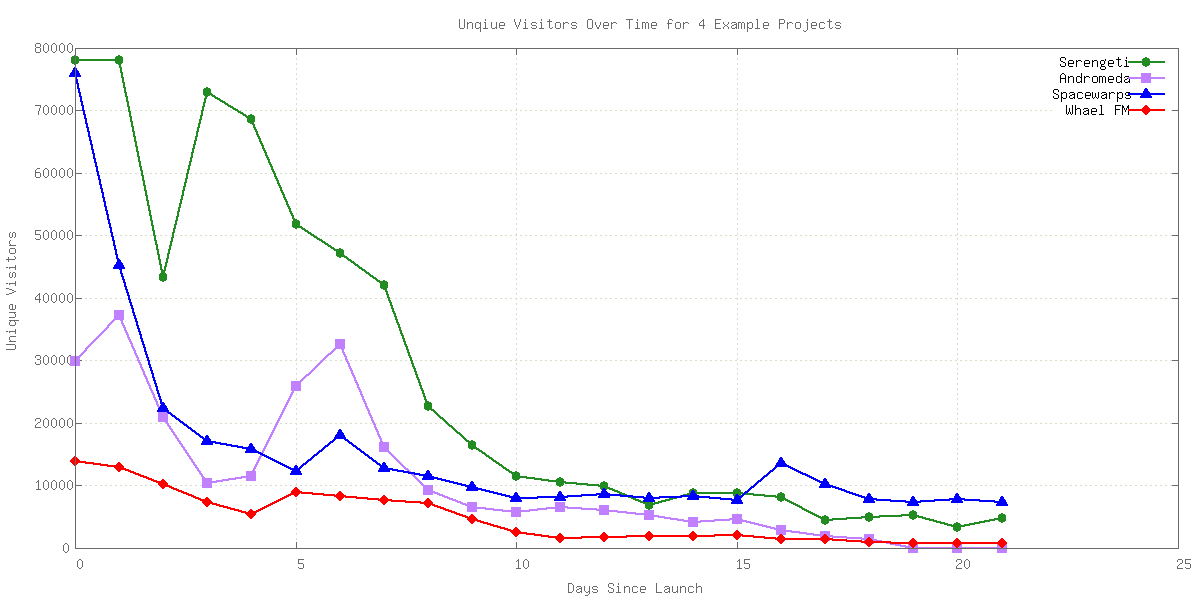
\includegraphics[width=0.50\textwidth]{data/launch-profiles/launch-profiles.png}
% \caption{\emph{Launch profiles for 4 example Zooniverse projects} - Displays the number of users per day for the first three weeks of four projects: Snapshot Serengeti, Andromeda Project, Space Warps, and Whale FM}
% \label{launchprofiles}
% \end{figure}

% % Andromeda, Whale FM, Spacewarps and Snapshot Serengeti as case studies

% The final theme we discuss here pertains to launching projects and outreach efforts, including the use of social media, newsletters, and other promotional material.

% It is a common misconception that websites are busy by default. Significant publicity and attention are often required to reach the right potential audiences for an online citizen science project. Networks and communities exist online to allow people to discover and share online projects, and are a valuable starting point for finding such individuals. The Zooniverse was one of the first organisations in this field and has grown a substantial network of people around it (\~ 860,000 at time of writing).

% Shown above in Figure \ref{launchprofiles} shows the number of users per day for the first three weeks of activity on four Zooniverse projects: Whale FM (Nov 2011), The Andromeda Project (Dec 2012), Snapshot Serengeti (Dec 2012) and Spacewarps (May 2013). Each project displays a subtly different profile of activity in its first days and weeks. Snapshot Serengeti and Space Warps enjoyed a healthy start of 80,000 users on launch day, mostly consisting of existing Zooniverse users (from other projects) responding to the launch announcement newsletter. % For example ... X and Y .... 

% As can be inferred from this, Zooniverse projects draw a substantial number of contributors from the pre-existing greater Zooniverse community. The Andromeda Project, mentioned above, was completed in a mere sixteen days thanks to a surge of activity from existing Zooniverse members, meaning all subjects were classified and tasks completed fully during this period.  Without this community, would have taken much longer.  Similarly, the initial surge in traffic on the Spacewarps project had 10,000 people contributing 500,000 classifications in its first twenty-four hours, and continued to sustain participation, with more than 10,000 people unique visitors daily even three weeks later, a majority of whom were seasoned ``Zooites''.  By comparison, it took weeks for blogs and news sites to pick up on the project and publish about it more widely.

% Thus, while a substantial quantity of useful work can be done by one-time visitors described earlier, having a core community propelled many of the later project launches, bringing quick attention and results faster than any normal recruitment mechanisms would have.  

% Zooniverse was not without its coverage in major media outlets, however, with the team benefiting from coverage in both traditional media outlets and online media, including international media networks such as the BBC (on \emph{The Sky At Night} and \emph{Click}), widely-read scientific magazines including regular coverage in the ``Citizen Science''` column of \emph{Scientific American}, and featured articles in \emph{National Geographic} \cite{zooniverse-natgeo}.  Such coverage regularly resulted in traffic spikes and influxes of new users.

% Beyond publicity, the Zooniverse team identified several factors that influence parcitipation at launch.  First, having a `Call to Action' appeared to improve retention; moreover, sites with less text, and clear, succinct front-page messages descriptions of a project had lower bounce rates overall.  This was first seen clearly with Planet Hunters but also with Galaxy Zoo's fourth incarnation. 


\section{Recommendations for Design}

\begin{table*}
\begin{center}
\begin{tabular}{p{4.5cm}p{13cm}}
Myth & Experience \\
\hline
\emph{Myth:} Adding pre-task tutorials boosts task performance & The Zooniverse team saw that tutorials increased \emph{bounce rates} dramatically, reducing the number of tasks completed per hour, with no perceived effect on performance; instead, \emph{in-task guidance} was more effective at getting individuals involved. \\
\hline
\emph{Myth:} Get users to sign up to join a project before starting a task & Forcing users to sign-up before participating also increased bounce rate; getting users involved in a real task before signing in lets them both do useful work and become familiarised to the tasks/project - ``try before buying in''. \\
\hline
\emph{Myth:} Experienced users perform better than new ones &  To the contrary, support was seen for this; no correlation between duration of use and user performance (e.g., \cite{simpson2013dynamic}). \\
\hline
\emph{Myth:} Citizen scientists become domain experts over time &  Related to a previous myth, any expertise gain is just as likely to include `false' expertise - that is, users might learn something about certain galaxies, while simultaneously learning fallacies about other galaxies, in which case they can hardly be said to be experts. \\
\hline
\emph{Myth:} Gameification motivates participation &  No, most of the reasons people participate in Zooniverse was `to help science'; gameification had no perceived effect \\
\hline
\emph{Myth:} The subjects need to be beautiful/interesting for people to be motivated & Relating to the last myth, intrinsic motivation is primarily to help science; interestingness/variability of subject is but one of many factors that can influence participation but is not a singular driver (e.g., \emph{Ice Hunters}). \\
\hline
\emph{Myth:} Include a `Don't know' button for skipping hard tasks &  No; introducing it allows people to give up; omitting it makes performing tasks more valuable \& encourages valuable partial solutions. \\
\hline
\emph{Myth:} Non-pictorial subjects are hard to understand/scary &  Several counter-examples, including \emph{Planet Hunters} in which users were given the ``raw'' light curve data with little explanation, yet seemed to offer no significant challenge. \\
\hline
\emph{Myth:} It's good to strip ``irrelevant'' context from data subjects to focus users on their tasks & Users enjoyed knowing where data came from, such as source ship and date in \emph{Old Weather} and season and region in \emph{Snapshot Serengeti}, and ``irrelevant'' side notes in \emph{Old Weather} logbooks brought people to the project and drove participation. \\
\hline
\emph{Myth:} ``If you build it, they will come'' &  Many factors contribute to whether citizen science programs attract users at launch; publicity, calls to action, having a clear purpose, and immediately engaging users. \\
\hline
\end{tabular}
\caption{\emph{Citizen Science Myths} - Common myths associated with designing for citizen science, with the Zooniverse team's perspectives on each.}
\label{tbl:myths}
\normalsize
\end{center}
\end{table*}

% the team is contiuing to work on making Zooniverse better
%   rigorous A-B testing of interface alternatives so that differences may be quantified (such as understanding the precise effect of interleaving dialogue prompts in the workflow)
%   controlled testing of different strategies for sustaining participation by varying scheduling of subjects
%      using favourites as a gauge of interestingness
% We summarised these observations in an series of ``myths'', or anti-patterns based on the observations made in this study.

% In the previous section, we described the key experiences that shaped the way the Zooniverse team regarded the design of projects, pertaining to supporting serendipitous discovery, sustaining engagement, and planning project launches. To form these themes into design recommendations, we re-visited the themes with the Zooniverse team, and performed a collective brainstorming to frame them in terms of \emph{anti-patterns} or misconceptions that might occur as by first-time citizen-science designers. (Patterns and anti-patterns are a frequently used method to  document design recommendations and justifications in complex design spaces, originating in architecture and used widely in software and UX design\cite{alexander2006pattern}.)  The result of this process are the ``myths'' of Table \ref{tbl:myths}.

In order to consolidate the themes just described into design recommendations, we re-visited them with the Zooniverse team to identify beliefs that they, themselves, or others in the field, thought were good ideas that were contradicted through experience.  These were consolidated into a set of \emph{anti-patterns} or ``myths of citizen science'', visible in Table \ref{tbl:myths}.  (Patterns and anti-patterns are a frequently used method to  document design recommendations and justifications in complex design spaces, originating in architecture and used widely in software and UX design \cite{alexander2006pattern}.)  While these recommendations may have been derived from personal experience and thus  should be translated

\section{Limitations and Future Work}
Pertaining to generalisability of our findings, it should be noted that, despite the diversity of fields represented by the Zooniverse projects, this analysis centred upon a single family of projects with common characteristics that may not pertain to other citizen science systems.  For example, the priority of all Zooniverse projects was \emph{scientific outcomes and discovery}, while other systems may have different, even multiple, priorities. Educating users, for instance, was not among the team's design goals, which was reflected in decisions such as reducing tutorials to minimum in-situ guidance to complete tasks.  While effective at increasing users' task time, this had the effect that users did not readily gain skill in task performance over time, as evidenced by a study showing that experienced users rarely outperformed new ones\cite{zooniverseblog}.  A second characteristic was that, as previously found \cite{raddick2010galaxy}, intrinsic motivation,  was responsible for the citizen participation among the Zooniverse projects.  This influenced strategic choices made by the team as to whether and how to communicate scientific milestones to participants,.  It was also seen to even inspire the science teams to conduct investigations and prepare articles expediently, as it was often felt that they ``owed it to the users'' to deliver on their commitment to publish results, given the dedication of the citizen community.  Finally a specific characteristic of Zooniverse is that, as described earlier, its tasks are focused on \emph{classification}, rather than data collection or problem solving.  While it is possible that our observations may generalise to other kinds of tasks, we refrain from making such claims given the complexity of understanding the many design dimensions of these systems.
% to provide frequent feedback to users about what their efforts have enabled

To enable the team to make more conclusive design recommendations, a current priority, is to introduce the capability to conduct effective low-cost A-B testing on interface design and interaction flow alternatives.  This capability will allow the team to quantitatively measure effects such as bounce rate, discussion adoption, among other metrics to evaluate detailed aspects of interface design and flow.  Measuring such effects may precisely characterise and guide the design process towards improved user experiences. 
%We have thus far refrained from reporting informal tests conducted because of the lack of such quantifiable certainty.  

%One area where such a testing framework will be useful is in optimising subject selection strategies during tasks for better sustaining user interest.  As described in the engagement section, users seem to be influenced by the variation and interesting-ness of subjects they are asked to classify.  The challenges are twofold; to figure out what subjects are interesting (or particularly uninteresting) to begin with, and then how to order or schedule these to users as they perform tasks.  Ideally, for example, user engagement might peak from a schedule that mixes yet unseen subjects (whose interestingness is yet unknown), with those who are known to be interesting (to pique user interest).

Looking forward, while the Zooniverse team achieved significant success with respect to enabling scientific discovery through the participation of its nearly million users, the team perceives that their investigation remains very unfinished.  For one, many significant challenges remain pertaining to improving the mechanisms and means by which citizens can initiate, lead and coordinate investigations.  In particular, given the autonomy demonstrated citizen volunteers towards carrying out their own investigations, the team are focusing on ways to open up access to both tools and data resources currently only available to the science team, so that these resources can be drawn upon in the process of citizen-led investigation.  One concrete milestone towards this goal was the first release of \emph{ZooTools}\footnote{ZooTools \url{tools.zooniverse.org/\#/dashboards/galaxy_zoo}}, a web interface that grants anyone direct access to the entire set of classifications in any of the Zooniverse projects.  Via ZooTools, users can explore all subjects in all databases and issue queries to extract certain ones with features, as only the science team previously could.  Previously, participants could only view subjects chosen by the system during tasks, and on secondhand accounts of subjects presented to others in the course of investigations.

Beyond giving participants better tools, the Zooniverse team has launched an experiment called \emph{Galaxy Zoo Quench} that puts makes citizens central to the entire academic journal article preparation process.  While still underway, Quench is only loosely guided by the science team, and milestones represent article article preparation progress, including analysing results, performing literature reviews, deriving relevant summaries, proofreading and integrating sections, and so on.  The success of this project and quality of its output may finally change the role of citizens to being engaged as true partners in the scientific process. 


% The degree of initiative demonstrated by citizens, across the Zooniverse projects, changed the way the Zooniverse team viewed the role of participants in citizen science systems from that of `volunteer workers' to partners in the scientific process.  To reflect this increased role, the team has committed development efforts to reducing the barriers that prevent citizen participants from carrying out their own investigations.  One such aspect of this is the development of a new suite of tools for granting users direct access to the entire Zooniverse classification databases as they are built, so that users can run arbitrary queries using a user-friendly web interface, called \emph{ZooTools}\footnote{ZooTools \url{tools.zooniverse.org/\#/dashboards/galaxy_zoo}}


% expanding the role of citizens beyond classification and informal discussion, to that of partners in a scientific collaboration.  To do this, the Zooniverse team has launched a new project and associated tools called \emph{Zooniverse Quench}\footnote{Zooniverse Quench \url{http://quench.zooniverse.org}} which 

%% TODO:  Quench early observations

%% FUTURE WORK
%% AUTOMATIC ONSET DETECTION FOR scientists
%% REPUTATION system - where there was someone who was very well spoken and loud, and writing technically
%% people have their own categorisation
%    if you email them they will be overload
%    SO, catch scientists them when they go to the site> CHECK OUT THIS DISCUSSION THREAD

% A-B testing alternatives - the cost of deriving two designs and 
% formally A-B testing them can be prohibitively expensive

% \section{Related work}

% galaxy_zoo\section{Conclusion}

\section{Acknowledgments}
Acknowledgments omitted for blind review.

\balance

%% elena notes
%%   actual task - functionality - the button was missing/feature was missing
%%   tutorial how do we teach them
%%   discussions
%%   launching projects
%%   sustaining engagements
%%     direct feedback
%%     effect of latency change on engagement?

%%   -----------
%%   punt :: deployment constriants on design  -- this is a real time systems
%%     and there are some specific feature sthat really need to go quickly
%%     it turned out that this combination worked well....
%%     any deployment engineer would have been able to figure out 

%% The Zooniverse framework team has derived significant has
%% been successively refined and scaled as the variety of tasks and
%% number of participants have increased.  At its current state,
%% currently having launched $X$ distinct applications for $Y$ scientific
%% domains, including astronomy, zoology, cell and marine biology,
%% archaeology and paleontology.  This platform represents a unique\cite{moore2011facebooking}


%%  These
%% applications, though separate, have been built on top 

%% The experiences from the first were used to derive design goals for
%% the next,

%% The contributions of the 
%% We identify key design challenges

%% especially as the best practices for designing citizen science systems
%% has not yet emerged.  Among the many design challenges include, being
%% able to appeal to participants with an extremely wide range of
%% expertise, ranging from no knowledge of the field to significant
%% background and interest.  Participants naturally feature a diversity
%% of natural competencies, which is manifested in some people being
%% simply much more adept at some tasks than others. Second, people have
%% many different reasons for engaging with citizen science projects, and
%% to sustain engagement, these platforms must appeal to, and engage
%% these different motivating reasons. Finally, there are a large variety
%% of issues pertaining to individual retention, well as supporting
%% various degrees of engagement -- from the ``sunday scientist'' to the
%% ``scienceoholic''.


%% The purpose of this examination of Zooniverse is to both to document
%% the experience gained from launches and iterations of the various
%% applications, comparing these experiences against previously
%% documented in other citizen-science projects.  The observations derive
%% from a lateral examination of the

%% The path from its first experimental app, Galaxy Zoo, to the 
%% twenty seven different projects that have launched on the Zooniverse project
%% required generalising the findings from the first project to different
%% kinds of tasks in other scientific domains.

%%  naturally Participants come from a wide
%% audience % with a massive variety of backgrounds and competencies,
%% such systems interface down to the workflow of how participants' input
%% is collated, verified, and provided as feedback to the participants,
%% along with the nature and kind(s) of affordances provided for
%% communicating and discussing remains challenigng

%% interfaces that have
%% appropriate affordances, the and features remains challenging, due
%% to the wide number of design considerations that mustbe taken
%% jointly into account.

%% Wide variety of expertise

% \section{Background: Brief History of Zooniverse}

% \emph{For the CSCW readers, outline the history of the development of the system
% including a detailed description}

% \section{Observations through iterations}

% \emph{I was thinking put key design observations here relating to how to cross-domain
% citizen science}

% If you want to use smaller typesetting for the reference list,
% uncomment the following line:
% \small


\bibliographystyle{acm-sigchi}
\bibliography{zooniverse-history}
\end{document}

%% from crw04
%% \begin{algorithm}[tb]
%%   \caption{Overview of our general negotiation process, which is common to all of our strategies.  Let $o_\text{own}$ and $o_\text{opp}$ represent our own and the opponent's latest offers, respectively. $t_c$ is the current time and $u_\tau$ is the aspiration level at time $t_c$.}\label{alg:generic-overview}
%%   \begin{algorithmic}
%%     \FOR{$t_c \in [0,1]$}
%%     \STATE $o_\text{opp} \Leftarrow $ {\sc ReceiveOffer}()
%%     \STATE $u_\tau \Leftarrow $ {\sc SetAspirationLevel}($o_\text{opp}, t_c$)
%%     \IF{{\sc GetUtility}($o_\text{opp}, t_c$) $\geq u_\tau$}
%%     \STATE {\sc AcceptOffer}($o_\text{opp}$)
%%     \RETURN
%%     \ENDIF
%%     \STATE $o_\text{own} \Leftarrow $ {\sc GenerateOffer}($u_\tau$)
%%     \STATE {\sc ProposeOffer}($o_\text{own}$)
%%     \ENDFOR
%%     \end{algorithmic}
%% \end{algorithm}

%%  LocalWords:  artefacts HCI artefact Dropbox Skydrive Google PDF
%%  LocalWords:  LaTeX versioning throughs interactional CDSSes UI LD
%%  LocalWords:  bioinformaticians iPad iCloud iCal favour favourite
%%  LocalWords:  microformats picoformats WebDAV situ VCS scm priori
%%  LocalWords:  Powerpoint CB's CBs each's bulleted parseable OTs
%%  LocalWords:  sub-schemas pre Dourish XLSX csv PPTX PPT ICS CalDAV
%%  LocalWords:  RSS VCF XSLT XLST CSS Dojo PNG


%% notes from Oxford, 22 August
%% SOCIAL MEDIA  > 
%% troubleshooting >> social media is used for troubleshooting
%% source of traffic >> we get a significant amount of traffic from social media
%%  whale.fm gets a lot of traffic from social media

%% INTERFACE >
%% Rising percent of tablet users > it needs to work on an ipad
%%  - ones that promote on the telly

%% Discussion forums >
%%    Why they were introduced
%%    How it evolved and emerged
%%       From "What's this?" to so much more!
%%       Increase engagement by letting people share pretty galaxies and discuss
%%        (basic statistics of how many people have done this)
   Key players / decisions - Moderators
%%       Independently tested hypothesis and moderators emerged as key mediators between participants and scientists
%%     Peas and verpwork 
%% Questions for Chris::
%%    _Key affordances of the forums w.r.t. how they facilitated these discussions_
%%    _Missing affordances - things that would have helped_
   _Role of project managers and scientists_
%%     What did they do to make things happen
%% Two path to science
%%   -> show -> classifications
%%           -> interesting things to talk about



% 

% what percentage of users are new versus old/existing users? 
% effects of email newsletters and things like that
% BBC the sky at night, BBC click, national geographic, 
% 

% Significant use of Twitter to advertise WormWatchLab at launch - Through Zooniverse accounts, science team accounts and subsequent retweets. Chris and Rob mentioned in Oxford that they send a newsletter to existing Zooniverse users to encourage them to take part in newly released projects, but social media use is essential to draw in outside users, which would otherwise rely on the Sky at Night, and the media, which many Citizen Science projects would not be able to draw on and which Zooniverse can only exploit on occasion. 

% Encouraging users to share subjects to pull in other users - See Snapshot Serengeti 'Save the Memes' campaign, which sought to raise funds but also to draw in other users, through memetic use of subjects. 

% In the initial interface, a button labeled ``discuss this'' on the classification interface was the primary method by which the discussion forums could be accessed.  To drive greater participation, the team experimented with several options for 

% The team examined the various ways in the interface that each of the projects linked users to discuss an item.  In several projects, a small speech bubble 'Bubbles' activities (TODO Clarify please), participants were asked to "confirm" "discuss" and "cancel" after each task.. % This is only true of the 'Bubbles' activity and not the 'Clouds' activity, which instead has a small speech bubble in the corner which users must click in order to discuss the image. No prompts are given at any point, although the tutorial does point the % speech bubble out to users.
% The options are now called "confirm" "discuss" and "cancel" as the interface asks "are you sure" after "submit" is selected. % This is only true of the 'Bubbles' activity and not the 'Clouds' activity, which instead has a small speech bubble in the corner which users must click in order to discuss the image. No prompts are given at any point, although the tutorial does point the % speech bubble out to users.
%  Citizen scientists who wish to contribute to the community in ways beyond simple classification have found other ways to do so. For example, Zooniverse discussion spaces are moderated not by the science team, but by volunteers, typically chosen from amongst those who participate in the beta test. Volunteer moderators have set community standards, produced substantial texts and guides for new participants and often act as a liaison between volunteers and science team, and it seems advantageous to distinguish between those providing expertise (typically the science team) within a community and those responsible for shaping and policing it. More recent projects have involved moderators and advanced users in the process of development; the Andromeda project includes Jules Wilkinson (moderator on Moon Zoo and Solar Stormwatch) as a full member of the project team, and Space Warps included XXXX of their likely volunteers in their initial workshop where the concept for the project was developed. 


% \subsection{Key components of a citizen science project}

% Despite the development of projects in very different domains of academic research, and which involve disparate user interactions, the core requirements for a successful citizen science project remain stable. A `main' interface allows a \emph{user} to complete a \emph{task} when presented with a \emph{subject}. The task is typically constrained by the tools provided (e.g. answer questions from a decision tree, mark craters on an image) and when completed typically results in the presentation of the next subject to be classified. In Zooniverse projects to date, participants perform tasks individually, and are typically not given control over choice of what subjects to work on. This latter choice makes deliberate manipulation of the data difficult and also ensures that project priorities are respected (i.e. it's not just the beautiful/interesting/easy subjects that are worked on). Secondly, some tutorial elements - either as a stand-alone tutorial, as an interactive within the interface or as surrounding context - are required to acquaint users with their tasks. An additional environment for discussion is typically, but not always, provided allowing for more free-form interaction between users and other participants such as scientists, developers and for which work goes beyond the initial task. Extra tools for manipulated subjects or for exploring contextual information may be provided in association with these discussion environments. 

%% One of Arfon's blog posts ties in nicely with the above "despite the development..." as it explains that fundamentally 
%% the team have tried to make it so that each project is the same 'deep down', differing only by goal and interface

% A community of participants is implicitly necessary for a citizen science project; crowdsourcing without a crowd is a perhaps unsolvable problem. However, levels of participation and involvement in the community will naturally vary; Zooniverse projects typically receive a substantial number of their classifications from users who will never return. A successful citizen science project will thus be designed to both enable these short-term participants to make useful contributions while still fostering longer-term engagement. This need also illustrates the requirement in most cases to assess the ability or accuracy of participants; many projects thus incorporate `tests', either explicitly or more commonly by including simulated or expert-classified subjects in the workflow presented to users. 

%% The Hcomp2013 "Volunteers' engagement in volunteer thinking project" paper states that for the Milky Way project, 78% of all
%% classifications are completed by regular users (i.e, those who return at least more than once) and for the Galaxy Zoo project
%% this value increases to 80%, which conflicts heavily with the above statements.

% \subsection{Task and Tutorial Design}
%% ask Chris about this
% What were the other problems with the forums??
% Blog post appears to conflict with the information above, which came from forums predominantly - implies that peas are NOT red... :|

% \subsubsection{Encouraging participation}

% (TODO: Neal - 
%  Value of fanboy/fangirling over beautiful Galaxies
%  Discussion of ``animal fans'' Snapshot Serengeti
%  TODO: Rob - do fans contribute more?)
%  Very first post is a pretty galaxy


%% Different prompts to talk.
%% Discussion of talk features. 

%% Galaxy Zoo Peas Corp and Hanny's Voorwerp.
%% Created Talk and then found cool planets in PH, Yellowballs tag in MWP, Convict Worm in Seafloor

% \subsection{Forums}
%% Forums -> 
%% Introduction of Talk 1.0 -> 
%% Introduction of Talk 2.0
%% Organisation and Fragmentation 
%% Top level organisation, moderators, scientists and how this has changed and impacted 

%% In a study investigating the effect of instructors on forum participation, Mazzolini and Maddison found that instructors who posted frequently on a forum on average produced shorter discussion threads \cite{mazzolini2003sage}. In the Zooniverse environment the participation of `moderators' and `scientists' could be hindering the discussion flow between general science citizens. Furthermore there was a negative correlation between instructor initiated conversations and participation, especially in the advanced units\cite{mazzolini2003sage}. 

%% @Neal does this support your findings so far?
%% Conversations started by moderators tend to be ignored
%% except in the case of particularly 'controversial' posts,
%% such as threads about the I don't know button. However,
%% such threads tend to be FAQ-style single post Q&A threads,
%% and so it's possible this is why. In fact 'welcome' style
%% threads are almost always started by moderators and these


%% threads are among the most popular threads across all projects.
%% However, certainly where moderators attempt to engage in
%% pre-existing discussion threads, their comments are ignored and
%% their questions go unanswered, except usually, by other
%% moderators, although this may partially be a result of the
%% subject matter or the time which has elapsed (necromancy). 

%% In terms of frequent posters, that's something I'll look into

%% Success stories: examples of super-moderators who externally test
%% contributions and distill them for the scientists
%% (why only in certain apps and not others?)
%% (how do super moderators affect the community // roles played)
%% Space Warps - Moderators and users teaching other users to use
%% modelling software to model subjects, in order to help
%% identify lenses. Seemingly entirely voluntarily, as posts point
%% out how unexpected these contributions were at this stage

%% http://www.galaxyzooforum.org/index.php?topic=264.msg10705#msg10705
%% Features a user making their first post, sharing a pretty subject

%% http://www.galaxyzooforum.org/index.php?topic=98.msg3529#msg3529
%% Features a user who is glad they joined, because of pretty subjects

%% Does not appear that users are spending extra time looking for
%% pretty or interesting or whatever galaxies, but rather transfer
%% these images into the forums after they're done doing their
%% ordinary classifying or after they happen across a particularly
%% exciting galaxy, but again while doing their ordinary classifying.




% when we turned on compulsory tutorial -- bounce rate went up

%% \subsection{Interface Design}
% Does good design improve participation?  Much evidence has suggested that \emph{good design builds trust}, by improving people's subjective appraisal of web sites and applications.  

%% Examples of surface level/aesthetic re-design >  (and perceived effects)
%% Moon Zoo : redesigned December 2011 - re-designed the web site around the interface, interface had a slight modifications, and perceived effect? % look to see if there was any effect? >> not as far as we can see

%% Examples of thematic redesign encompassing addition of narrative context (and percevied effect) > 
%% How to measure engagement
%%   how much time spent on the site
%%   people stick over a minute, (2-3 mins, high is 20)
%%   (moderators of old weather)?
  % TODO: can we say anything about the effect of the narrative in Old Weather? 
  % evidence in the discussion forums ? 
  %   > i wonder why the handwriting has changed?
  %   > most keen to help each other out -- 

%% Examples of interface affordance design (and perceived effect)
%% GZ / GZ2 - so it was turned into a deicsion tree
%%   what kind of galaxy, 6 buttons -> decision tree

% much better data, and it decreased participation

% I DONT KNOW button - don't have one (blog post)
  
